\documentclass[twoside]{book}

% Packages required by doxygen
\usepackage{fixltx2e}
\usepackage{calc}
\usepackage{doxygen}
\usepackage[export]{adjustbox} % also loads graphicx
\usepackage{graphicx}
\usepackage[utf8]{inputenc}
\usepackage{makeidx}
\usepackage{multicol}
\usepackage{multirow}
\PassOptionsToPackage{warn}{textcomp}
\usepackage{textcomp}
\usepackage[nointegrals]{wasysym}
\usepackage[table]{xcolor}

% NLS support packages
\usepackage[spanish]{babel}
% Font selection
\usepackage[T1]{fontenc}
\usepackage[scaled=.90]{helvet}
\usepackage{courier}
\usepackage{amssymb}
\usepackage{sectsty}
\renewcommand{\familydefault}{\sfdefault}
\allsectionsfont{%
  \fontseries{bc}\selectfont%
  \color{darkgray}%
}
\renewcommand{\DoxyLabelFont}{%
  \fontseries{bc}\selectfont%
  \color{darkgray}%
}
\newcommand{\+}{\discretionary{\mbox{\scriptsize$\hookleftarrow$}}{}{}}

% Page & text layout
\usepackage{geometry}
\geometry{%
  a4paper,%
  top=2.5cm,%
  bottom=2.5cm,%
  left=2.5cm,%
  right=2.5cm%
}
\tolerance=750
\hfuzz=15pt
\hbadness=750
\setlength{\emergencystretch}{15pt}
\setlength{\parindent}{0cm}
\setlength{\parskip}{3ex plus 2ex minus 2ex}
\makeatletter
\renewcommand{\paragraph}{%
  \@startsection{paragraph}{4}{0ex}{-1.0ex}{1.0ex}{%
    \normalfont\normalsize\bfseries\SS@parafont%
  }%
}
\renewcommand{\subparagraph}{%
  \@startsection{subparagraph}{5}{0ex}{-1.0ex}{1.0ex}{%
    \normalfont\normalsize\bfseries\SS@subparafont%
  }%
}
\makeatother

% Headers & footers
\usepackage{fancyhdr}
\pagestyle{fancyplain}
\fancyhead[LE]{\fancyplain{}{\bfseries\thepage}}
\fancyhead[CE]{\fancyplain{}{}}
\fancyhead[RE]{\fancyplain{}{\bfseries\leftmark}}
\fancyhead[LO]{\fancyplain{}{\bfseries\rightmark}}
\fancyhead[CO]{\fancyplain{}{}}
\fancyhead[RO]{\fancyplain{}{\bfseries\thepage}}
\fancyfoot[LE]{\fancyplain{}{}}
\fancyfoot[CE]{\fancyplain{}{}}
\fancyfoot[RE]{\fancyplain{}{\bfseries\scriptsize Generado por Doxygen }}
\fancyfoot[LO]{\fancyplain{}{\bfseries\scriptsize Generado por Doxygen }}
\fancyfoot[CO]{\fancyplain{}{}}
\fancyfoot[RO]{\fancyplain{}{}}
\renewcommand{\footrulewidth}{0.4pt}
\renewcommand{\chaptermark}[1]{%
  \markboth{#1}{}%
}
\renewcommand{\sectionmark}[1]{%
  \markright{\thesection\ #1}%
}

% Indices & bibliography
\usepackage{natbib}
\usepackage[titles]{tocloft}
\setcounter{tocdepth}{3}
\setcounter{secnumdepth}{5}
\makeindex

% Hyperlinks (required, but should be loaded last)
\usepackage{ifpdf}
\ifpdf
  \usepackage[pdftex,pagebackref=true]{hyperref}
\else
  \usepackage[ps2pdf,pagebackref=true]{hyperref}
\fi
\hypersetup{%
  colorlinks=true,%
  linkcolor=blue,%
  citecolor=blue,%
  unicode%
}

% Custom commands
\newcommand{\clearemptydoublepage}{%
  \newpage{\pagestyle{empty}\cleardoublepage}%
}

\usepackage{caption}
\captionsetup{labelsep=space,justification=centering,font={bf},singlelinecheck=off,skip=4pt,position=top}

%===== C O N T E N T S =====

\begin{document}

% Titlepage & ToC
\hypersetup{pageanchor=false,
             bookmarksnumbered=true,
             pdfencoding=unicode
            }
\pagenumbering{alph}
\begin{titlepage}
\vspace*{7cm}
\begin{center}%
{\Large Práctica de P\+R\+O2 (Primavera 2020)\+: Árboles Filogenéticos \\[1ex]\large Jia Long Ji Qiu -\/ 20-\/05-\/2020 }\\
\vspace*{1cm}
{\large Generado por Doxygen 1.8.13}\\
\end{center}
\end{titlepage}
\clearemptydoublepage
\pagenumbering{roman}
\tableofcontents
\clearemptydoublepage
\pagenumbering{arabic}
\hypersetup{pageanchor=true}

%--- Begin generated contents ---
\chapter{Práctica de P\+R\+O2 (Primavera 2020)\+: Árboles filogenéticos. Documentación}
\label{index}\hypertarget{index}{}El programa principal se encuentra en el módulo \hyperlink{program_8cc}{program.\+cc}. Acorde a la datos sugeridos por el enunciado, se han implementado los módulos \hyperlink{class_especie}{Especie}, para representar cada especie con sus respectivos atributos, \hyperlink{class_cjt___especies}{Cjt\+\_\+\+Especies}, donde se guardan las especies y la relación entre ellas, y \hyperlink{class_cjt___clusters}{Cjt\+\_\+\+Clusters}, donde se desarrolla la agrupación de especies dentro de un conjunto de especies. 
\chapter{Índice de clases}
\section{Lista de clases}
Lista de las clases, estructuras, uniones e interfaces con una breve descripción\+:\begin{DoxyCompactList}
\item\contentsline{section}{\hyperlink{class_cjt___clusters}{Cjt\+\_\+\+Clusters} \\*Representa la información y las operaciones de un conjunto de clústers }{\pageref{class_cjt___clusters}}{}
\item\contentsline{section}{\hyperlink{class_cjt___especies}{Cjt\+\_\+\+Especies} \\*Representa la información y las operaciones asociadas a un conjunto de especies }{\pageref{class_cjt___especies}}{}
\item\contentsline{section}{\hyperlink{class_especie}{Especie} \\*Representa la información y las operaciones asociadas a una especie }{\pageref{class_especie}}{}
\end{DoxyCompactList}

\chapter{Indice de archivos}
\section{Lista de archivos}
Lista de todos los archivos con descripciones breves\+:\begin{DoxyCompactList}
\item\contentsline{section}{\hyperlink{_cjt___clusters_8cc}{Cjt\+\_\+\+Clusters.\+cc} \\*Código de la clase \hyperlink{class_cjt___clusters}{Cjt\+\_\+\+Clusters} }{\pageref{_cjt___clusters_8cc}}{}
\item\contentsline{section}{\hyperlink{_cjt___clusters_8hh}{Cjt\+\_\+\+Clusters.\+hh} \\*Especificación de la clase \hyperlink{class_cjt___clusters}{Cjt\+\_\+\+Clusters} }{\pageref{_cjt___clusters_8hh}}{}
\item\contentsline{section}{\hyperlink{_cjt___especies_8cc}{Cjt\+\_\+\+Especies.\+cc} \\*Código de la clase \hyperlink{class_cjt___especies}{Cjt\+\_\+\+Especies} }{\pageref{_cjt___especies_8cc}}{}
\item\contentsline{section}{\hyperlink{_cjt___especies_8hh}{Cjt\+\_\+\+Especies.\+hh} \\*Especificación de la clase \hyperlink{class_cjt___especies}{Cjt\+\_\+\+Especies} }{\pageref{_cjt___especies_8hh}}{}
\item\contentsline{section}{\hyperlink{_especie_8cc}{Especie.\+cc} \\*Código de la clase \hyperlink{class_especie}{Especie} }{\pageref{_especie_8cc}}{}
\item\contentsline{section}{\hyperlink{_especie_8hh}{Especie.\+hh} \\*Especificación de la clase \hyperlink{class_especie}{Especie} }{\pageref{_especie_8hh}}{}
\item\contentsline{section}{\hyperlink{program_8cc}{program.\+cc} \\*Programa principal }{\pageref{program_8cc}}{}
\end{DoxyCompactList}

\chapter{Documentación de las clases}
\hypertarget{class_cjt___clusters}{}\section{Referencia de la Clase Cjt\+\_\+\+Clusters}
\label{class_cjt___clusters}\index{Cjt\+\_\+\+Clusters@{Cjt\+\_\+\+Clusters}}


Representa la información y las operaciones de un conjunto de clústers.  


\subsection*{Métodos públicos}
\begin{DoxyCompactItemize}
\item 
\hyperlink{class_cjt___clusters_a2e55759944a78043744103e19dd87c1c}{Cjt\+\_\+\+Clusters} ()
\begin{DoxyCompactList}\small\item\em Constructora por defecto. \end{DoxyCompactList}\item 
\hyperlink{class_cjt___clusters_a11e683ee54988d48d34c9cb2f6d52be6}{Cjt\+\_\+\+Clusters} (const \hyperlink{class_cjt___especies}{Cjt\+\_\+\+Especies} \&e)
\begin{DoxyCompactList}\small\item\em Constructora a partir de un conjunto de especies. \end{DoxyCompactList}\item 
void \hyperlink{class_cjt___clusters_a4675196f92740eda90fcbdf7942ee04b}{ejecutar\+\_\+paso\+\_\+wpgma} (bool \&b)
\begin{DoxyCompactList}\small\item\em Ejecuta un paso del algoritmo W\+P\+G\+MA. \end{DoxyCompactList}\item 
void \hyperlink{class_cjt___clusters_add140d48281573802396c267f0d15cee}{imprimir\+\_\+cluster} (string id, bool \&b) const
\begin{DoxyCompactList}\small\item\em Escritura de un clúster del conjunto, dado un identificador. \end{DoxyCompactList}\item 
void \hyperlink{class_cjt___clusters_a289dfd3307b383620edc1f901dced7b0}{imprimir\+\_\+arbol\+\_\+filogenetico} (bool \&b)
\begin{DoxyCompactList}\small\item\em Escritura del árbol filogenético del conjunto de especies con el que se ha inicializado el conjunto de clústers. \end{DoxyCompactList}\item 
void \hyperlink{class_cjt___clusters_a8caa8d4eae15730feccea2ce7d22a196}{imprimir\+\_\+distancias\+\_\+c} () const
\begin{DoxyCompactList}\small\item\em Escritura de la tabla de distancias entre clústers. \end{DoxyCompactList}\end{DoxyCompactItemize}
\subsection*{Métodos privados}
\begin{DoxyCompactItemize}
\item 
void \hyperlink{class_cjt___clusters_ac0e4dd151f0bbd2954d44551330a8757}{distancia\+\_\+minima} ()
\begin{DoxyCompactList}\small\item\em Calcula la distancia mínima entre los clústers del conjunto. \end{DoxyCompactList}\item 
void \hyperlink{class_cjt___clusters_a04cfe3b7b8998398a48459f9a9339c22}{algoritmo\+\_\+wpgma} ()
\begin{DoxyCompactList}\small\item\em Ejecuta un paso del algoritmo W\+P\+G\+MA. \end{DoxyCompactList}\end{DoxyCompactItemize}
\subsection*{Atributos privados}
\begin{DoxyCompactItemize}
\item 
map$<$ string, map$<$ string, double $>$ $>$ \hyperlink{class_cjt___clusters_a2b912c7987fd370bdeaf5dabb966240f}{distancias\+\_\+c}
\begin{DoxyCompactList}\small\item\em Mapa de submapas donde se guardan las distancias entre dos especies, cuyos identificadores son las keys. \end{DoxyCompactList}\item 
map$<$ string, Bin\+Tree$<$ pair$<$ string, double $>$ $>$ $>$ \hyperlink{class_cjt___clusters_a866c5a14f8f50598be2af9fd8c115dd2}{clusters}
\begin{DoxyCompactList}\small\item\em Mapa de árboles binarios donde se guardan los clústers, donde la key de cada árbol es el identificador de su nodo. \end{DoxyCompactList}\item 
string \hyperlink{class_cjt___clusters_af010e61859190999fb23f1854f4d23aa}{save\+\_\+c1}
\begin{DoxyCompactList}\small\item\em Parámetro auxiliar que indica el identificador de uno de los dos clústers de distancia mínima, dicho identificador es el menor. \end{DoxyCompactList}\item 
string \hyperlink{class_cjt___clusters_a1406c60345958da0016fa3c0b1cd89f5}{save\+\_\+c2}
\begin{DoxyCompactList}\small\item\em Parámetro auxiliar que indica el identificador de uno de los dos clústers de distancia mínima, dicho identificador es el mayor. \end{DoxyCompactList}\item 
double \hyperlink{class_cjt___clusters_a1b94b5f25778ee95796a9be966f1c619}{d\+\_\+min}
\begin{DoxyCompactList}\small\item\em Parámetro auxiliar que indica la distancia mínima entre el clúster save\+\_\+c1 y save\+\_\+c2. \end{DoxyCompactList}\end{DoxyCompactItemize}


\subsection{Descripción detallada}
Representa la información y las operaciones de un conjunto de clústers. 

Sus operaciones son la modificadora de ejecución de un paso del algoritmo W\+P\+G\+MA, y las de escritura de un clúster dado un identificador, del árbol filogenético del conjunto de clústers y de la tabla de distancias entre los clústers del conjunto

Hay declaradas varias operaciones auxiliares como {\itshape private} 

Definición en la línea 21 del archivo Cjt\+\_\+\+Clusters.\+hh.



\subsection{Documentación del constructor y destructor}
\mbox{\Hypertarget{class_cjt___clusters_a2e55759944a78043744103e19dd87c1c}\label{class_cjt___clusters_a2e55759944a78043744103e19dd87c1c}} 
\index{Cjt\+\_\+\+Clusters@{Cjt\+\_\+\+Clusters}!Cjt\+\_\+\+Clusters@{Cjt\+\_\+\+Clusters}}
\index{Cjt\+\_\+\+Clusters@{Cjt\+\_\+\+Clusters}!Cjt\+\_\+\+Clusters@{Cjt\+\_\+\+Clusters}}
\subsubsection{\texorpdfstring{Cjt\+\_\+\+Clusters()}{Cjt\_Clusters()}\hspace{0.1cm}{\footnotesize\ttfamily [1/2]}}
{\footnotesize\ttfamily Cjt\+\_\+\+Clusters\+::\+Cjt\+\_\+\+Clusters (\begin{DoxyParamCaption}{ }\end{DoxyParamCaption})}



Constructora por defecto. 

\begin{DoxyPrecond}{Precondición}
Cierto 
\end{DoxyPrecond}
\begin{DoxyPostcond}{Postcondición}
Se ha creado un conjunto de clusters vacío 
\end{DoxyPostcond}


Definición en la línea 6 del archivo Cjt\+\_\+\+Clusters.\+cc.


\begin{DoxyCode}
6 \{\}
\end{DoxyCode}
\mbox{\Hypertarget{class_cjt___clusters_a11e683ee54988d48d34c9cb2f6d52be6}\label{class_cjt___clusters_a11e683ee54988d48d34c9cb2f6d52be6}} 
\index{Cjt\+\_\+\+Clusters@{Cjt\+\_\+\+Clusters}!Cjt\+\_\+\+Clusters@{Cjt\+\_\+\+Clusters}}
\index{Cjt\+\_\+\+Clusters@{Cjt\+\_\+\+Clusters}!Cjt\+\_\+\+Clusters@{Cjt\+\_\+\+Clusters}}
\subsubsection{\texorpdfstring{Cjt\+\_\+\+Clusters()}{Cjt\_Clusters()}\hspace{0.1cm}{\footnotesize\ttfamily [2/2]}}
{\footnotesize\ttfamily Cjt\+\_\+\+Clusters\+::\+Cjt\+\_\+\+Clusters (\begin{DoxyParamCaption}\item[{const \hyperlink{class_cjt___especies}{Cjt\+\_\+\+Especies} \&}]{e }\end{DoxyParamCaption})}



Constructora a partir de un conjunto de especies. 

\begin{DoxyPrecond}{Precondición}
Cierto 
\end{DoxyPrecond}
\begin{DoxyPostcond}{Postcondición}
Se ha creado un conjunto de clusters a partir de un conjunto de especies e. Se le asigna al parámetro implícito los clústers y sus distancias obtenidas a partir de e. 
\end{DoxyPostcond}


Definición en la línea 8 del archivo Cjt\+\_\+\+Clusters.\+cc.


\begin{DoxyCode}
8                                                 \{
9   \hyperlink{class_cjt___clusters_a1b94b5f25778ee95796a9be966f1c619}{d\_min} = -1;
10   \textcolor{keywordtype}{int} size = e.\hyperlink{class_cjt___especies_a7061cb2108f9be2b12b8f2c5ae99a82d}{size}();
11   \textcolor{keywordflow}{for} (\textcolor{keywordtype}{int} i = 0; i < size; ++i) \{
12     \textcolor{keywordtype}{string} \textcolor{keywordtype}{id} = e.\hyperlink{class_cjt___especies_a0cc233873c53e5120cd362de7821eb16}{consultar\_id\_iesimo}(i);
13     BinTree<pair<string, double> > leaf(make\_pair(\textcolor{keywordtype}{id}, -1));
14     \hyperlink{class_cjt___clusters_a866c5a14f8f50598be2af9fd8c115dd2}{clusters}.insert(\hyperlink{class_cjt___clusters_a866c5a14f8f50598be2af9fd8c115dd2}{clusters}.end(), make\_pair(\textcolor{keywordtype}{id}, leaf));
15   \}
16   map<string, double> aux;
17   map<string, BinTree<pair<string, double> > >::iterator it1 = \hyperlink{class_cjt___clusters_a866c5a14f8f50598be2af9fd8c115dd2}{clusters}.begin();
18   \textcolor{keywordflow}{while} (it1 != \hyperlink{class_cjt___clusters_a866c5a14f8f50598be2af9fd8c115dd2}{clusters}.end()) \{
19     map<string, double> aux;
20     map<string, BinTree<pair<string, double> > >::iterator it2 = it1;
21     ++it2;
22     \textcolor{keywordflow}{while} (it2 != \hyperlink{class_cjt___clusters_a866c5a14f8f50598be2af9fd8c115dd2}{clusters}.end()) \{
23       \textcolor{keywordtype}{string} id1 = it1->first;
24       \textcolor{keywordtype}{string} id2 = it2->first;
25       \textcolor{keywordtype}{double} d = e.\hyperlink{class_cjt___especies_a55f41bd03feccf515a491abca95bd60f}{consultar\_distancia}(id1, id2);
26       aux.insert(aux.end(), make\_pair(id2, d));
27       ++it2;
28     \}
29     \hyperlink{class_cjt___clusters_a2b912c7987fd370bdeaf5dabb966240f}{distancias\_c}.insert(\hyperlink{class_cjt___clusters_a2b912c7987fd370bdeaf5dabb966240f}{distancias\_c}.end(), make\_pair(it1->first, aux));
30     ++it1;
31   \}
32   \hyperlink{class_cjt___clusters_ac0e4dd151f0bbd2954d44551330a8757}{distancia\_minima}();
33 \}
\end{DoxyCode}


\subsection{Documentación de las funciones miembro}
\mbox{\Hypertarget{class_cjt___clusters_a4675196f92740eda90fcbdf7942ee04b}\label{class_cjt___clusters_a4675196f92740eda90fcbdf7942ee04b}} 
\index{Cjt\+\_\+\+Clusters@{Cjt\+\_\+\+Clusters}!ejecutar\+\_\+paso\+\_\+wpgma@{ejecutar\+\_\+paso\+\_\+wpgma}}
\index{ejecutar\+\_\+paso\+\_\+wpgma@{ejecutar\+\_\+paso\+\_\+wpgma}!Cjt\+\_\+\+Clusters@{Cjt\+\_\+\+Clusters}}
\subsubsection{\texorpdfstring{ejecutar\+\_\+paso\+\_\+wpgma()}{ejecutar\_paso\_wpgma()}}
{\footnotesize\ttfamily void Cjt\+\_\+\+Clusters\+::ejecutar\+\_\+paso\+\_\+wpgma (\begin{DoxyParamCaption}\item[{bool \&}]{b }\end{DoxyParamCaption})}



Ejecuta un paso del algoritmo W\+P\+G\+MA. 

\begin{DoxyPrecond}{Precondición}
Cierto 
\end{DoxyPrecond}
\begin{DoxyPostcond}{Postcondición}
b indica si el número de clústers del parámetro implícito es mayor que 1; si b = true, se ha ejecutado un paso del algoritmo W\+P\+G\+MA; b = false contrariamente 
\end{DoxyPostcond}


Definición en la línea 141 del archivo Cjt\+\_\+\+Clusters.\+cc.


\begin{DoxyCode}
141                                               \{
142   \textcolor{keywordflow}{if} (\hyperlink{class_cjt___clusters_a866c5a14f8f50598be2af9fd8c115dd2}{clusters}.size() > 1) \{
143     b = \textcolor{keyword}{true};
144     \hyperlink{class_cjt___clusters_a04cfe3b7b8998398a48459f9a9339c22}{algoritmo\_wpgma}();
145     \hyperlink{_cjt___clusters_8cc_a5cec9117fc9081104f0adb60b07b64e5}{imprimir\_tabla}(\hyperlink{class_cjt___clusters_a2b912c7987fd370bdeaf5dabb966240f}{distancias\_c});
146   \}
147   \textcolor{keywordflow}{else} b = \textcolor{keyword}{false};
148 \}
\end{DoxyCode}
\mbox{\Hypertarget{class_cjt___clusters_add140d48281573802396c267f0d15cee}\label{class_cjt___clusters_add140d48281573802396c267f0d15cee}} 
\index{Cjt\+\_\+\+Clusters@{Cjt\+\_\+\+Clusters}!imprimir\+\_\+cluster@{imprimir\+\_\+cluster}}
\index{imprimir\+\_\+cluster@{imprimir\+\_\+cluster}!Cjt\+\_\+\+Clusters@{Cjt\+\_\+\+Clusters}}
\subsubsection{\texorpdfstring{imprimir\+\_\+cluster()}{imprimir\_cluster()}}
{\footnotesize\ttfamily void Cjt\+\_\+\+Clusters\+::imprimir\+\_\+cluster (\begin{DoxyParamCaption}\item[{string}]{id,  }\item[{bool \&}]{b }\end{DoxyParamCaption}) const}



Escritura de un clúster del conjunto, dado un identificador. 

\begin{DoxyPrecond}{Precondición}
El parámetro implícito está inicializado 
\end{DoxyPrecond}
\begin{DoxyPostcond}{Postcondición}
b indica si el parámetro implícito contiene un clúster con el identificador id dado; si b = true, se escribe dicho clúster por el canal estándar de salida; b = false contrariamente 
\end{DoxyPostcond}


Definición en la línea 163 del archivo Cjt\+\_\+\+Clusters.\+cc.


\begin{DoxyCode}
163                                                             \{
164   map<string, BinTree<pair<string,double> > >::const\_iterator it = \hyperlink{class_cjt___clusters_a866c5a14f8f50598be2af9fd8c115dd2}{clusters}.find(\textcolor{keywordtype}{id});
165   \textcolor{keywordflow}{if} (it == \hyperlink{class_cjt___clusters_a866c5a14f8f50598be2af9fd8c115dd2}{clusters}.end()) b = \textcolor{keyword}{false};
166   \textcolor{keywordflow}{else} \{
167     b = \textcolor{keyword}{true};
168     \hyperlink{_cjt___clusters_8cc_a4afe93558c94b1dce66fff0cf68cb08a}{imprimir\_preorden}(it->second);
169     cout << endl;
170   \}
171 \}
\end{DoxyCode}
\mbox{\Hypertarget{class_cjt___clusters_a289dfd3307b383620edc1f901dced7b0}\label{class_cjt___clusters_a289dfd3307b383620edc1f901dced7b0}} 
\index{Cjt\+\_\+\+Clusters@{Cjt\+\_\+\+Clusters}!imprimir\+\_\+arbol\+\_\+filogenetico@{imprimir\+\_\+arbol\+\_\+filogenetico}}
\index{imprimir\+\_\+arbol\+\_\+filogenetico@{imprimir\+\_\+arbol\+\_\+filogenetico}!Cjt\+\_\+\+Clusters@{Cjt\+\_\+\+Clusters}}
\subsubsection{\texorpdfstring{imprimir\+\_\+arbol\+\_\+filogenetico()}{imprimir\_arbol\_filogenetico()}}
{\footnotesize\ttfamily void Cjt\+\_\+\+Clusters\+::imprimir\+\_\+arbol\+\_\+filogenetico (\begin{DoxyParamCaption}\item[{bool \&}]{b }\end{DoxyParamCaption})}



Escritura del árbol filogenético del conjunto de especies con el que se ha inicializado el conjunto de clústers. 

\begin{DoxyPrecond}{Precondición}
Cierto 
\end{DoxyPrecond}
\begin{DoxyPostcond}{Postcondición}
b indica si el conjunto de clústers está vacío. Si b = false, se escribe el árbol filogenético (en preorden) del conjunto actual de clusters. El parámetro implícito pasa a tener el conjunto final de clústers, resultado de aplicar el algoritmo W\+P\+G\+MA de manera completa 
\end{DoxyPostcond}


Definición en la línea 173 del archivo Cjt\+\_\+\+Clusters.\+cc.


\begin{DoxyCode}
173                                                       \{
174 
175   \textcolor{keywordflow}{if} (\hyperlink{class_cjt___clusters_a866c5a14f8f50598be2af9fd8c115dd2}{clusters}.size() == 0) b = \textcolor{keyword}{true};
176   \textcolor{keywordflow}{else} \{
177     b = \textcolor{keyword}{false};
178     \textcolor{keywordflow}{while} (\hyperlink{class_cjt___clusters_a866c5a14f8f50598be2af9fd8c115dd2}{clusters}.size() > 1) \{
179       \hyperlink{class_cjt___clusters_a04cfe3b7b8998398a48459f9a9339c22}{algoritmo\_wpgma}();
180     \}
181     \hyperlink{_cjt___clusters_8cc_a4afe93558c94b1dce66fff0cf68cb08a}{imprimir\_preorden}(\hyperlink{class_cjt___clusters_a866c5a14f8f50598be2af9fd8c115dd2}{clusters}.begin()->second);
182     cout << endl;
183   \}
184 \}
\end{DoxyCode}
\mbox{\Hypertarget{class_cjt___clusters_a8caa8d4eae15730feccea2ce7d22a196}\label{class_cjt___clusters_a8caa8d4eae15730feccea2ce7d22a196}} 
\index{Cjt\+\_\+\+Clusters@{Cjt\+\_\+\+Clusters}!imprimir\+\_\+distancias\+\_\+c@{imprimir\+\_\+distancias\+\_\+c}}
\index{imprimir\+\_\+distancias\+\_\+c@{imprimir\+\_\+distancias\+\_\+c}!Cjt\+\_\+\+Clusters@{Cjt\+\_\+\+Clusters}}
\subsubsection{\texorpdfstring{imprimir\+\_\+distancias\+\_\+c()}{imprimir\_distancias\_c()}}
{\footnotesize\ttfamily void Cjt\+\_\+\+Clusters\+::imprimir\+\_\+distancias\+\_\+c (\begin{DoxyParamCaption}{ }\end{DoxyParamCaption}) const}



Escritura de la tabla de distancias entre clústers. 

\begin{DoxyPrecond}{Precondición}
Cierto 
\end{DoxyPrecond}
\begin{DoxyPostcond}{Postcondición}
Se ha escrito en el canal estándar de salida la tabla de distancias del parámetro implícito 
\end{DoxyPostcond}


Definición en la línea 186 del archivo Cjt\+\_\+\+Clusters.\+cc.


\begin{DoxyCode}
186                                                \{
187   \hyperlink{_cjt___clusters_8cc_a5cec9117fc9081104f0adb60b07b64e5}{imprimir\_tabla}(\hyperlink{class_cjt___clusters_a2b912c7987fd370bdeaf5dabb966240f}{distancias\_c});
188 \}
\end{DoxyCode}
\mbox{\Hypertarget{class_cjt___clusters_ac0e4dd151f0bbd2954d44551330a8757}\label{class_cjt___clusters_ac0e4dd151f0bbd2954d44551330a8757}} 
\index{Cjt\+\_\+\+Clusters@{Cjt\+\_\+\+Clusters}!distancia\+\_\+minima@{distancia\+\_\+minima}}
\index{distancia\+\_\+minima@{distancia\+\_\+minima}!Cjt\+\_\+\+Clusters@{Cjt\+\_\+\+Clusters}}
\subsubsection{\texorpdfstring{distancia\+\_\+minima()}{distancia\_minima()}}
{\footnotesize\ttfamily void Cjt\+\_\+\+Clusters\+::distancia\+\_\+minima (\begin{DoxyParamCaption}{ }\end{DoxyParamCaption})\hspace{0.3cm}{\ttfamily [private]}}



Calcula la distancia mínima entre los clústers del conjunto. 

\begin{DoxyPrecond}{Precondición}
Cierto 
\end{DoxyPrecond}
\begin{DoxyPostcond}{Postcondición}
Se atribuyen a \textquotesingle{}save\+\_\+c1\textquotesingle{} y \textquotesingle{}save\+\_\+c2\textquotesingle{} (tal que save\+\_\+c1 $<$ save\+\_\+c2) los identificadores de los clusters cuya distancia es la mínima. \textquotesingle{}d\+\_\+min\textquotesingle{} es dicha distancia. 
\end{DoxyPostcond}


Definición en la línea 35 del archivo Cjt\+\_\+\+Clusters.\+cc.


\begin{DoxyCode}
35                                     \{
36   map<string, map<string, double> >::const\_iterator it1 = \hyperlink{class_cjt___clusters_a2b912c7987fd370bdeaf5dabb966240f}{distancias\_c}.begin();
37   \textcolor{keywordflow}{while} (it1 != \hyperlink{class_cjt___clusters_a2b912c7987fd370bdeaf5dabb966240f}{distancias\_c}.end()) \{
38     map<string, double>::const\_iterator it2 = it1->second.begin();
39     \textcolor{keywordflow}{while} (it2 != it1->second.end()) \{
40       \textcolor{keywordtype}{double} d = it2->second;
41       \textcolor{keywordflow}{if} (\hyperlink{class_cjt___clusters_a1b94b5f25778ee95796a9be966f1c619}{d\_min} == -1 or d < \hyperlink{class_cjt___clusters_a1b94b5f25778ee95796a9be966f1c619}{d\_min}) \{
42         \hyperlink{class_cjt___clusters_af010e61859190999fb23f1854f4d23aa}{save\_c1} = it1->first;
43         \hyperlink{class_cjt___clusters_a1406c60345958da0016fa3c0b1cd89f5}{save\_c2} = it2->first;
44         \hyperlink{class_cjt___clusters_a1b94b5f25778ee95796a9be966f1c619}{d\_min} = d;
45       \}
46       ++it2;
47     \}
48     ++it1;
49   \}
50 \}
\end{DoxyCode}
\mbox{\Hypertarget{class_cjt___clusters_a04cfe3b7b8998398a48459f9a9339c22}\label{class_cjt___clusters_a04cfe3b7b8998398a48459f9a9339c22}} 
\index{Cjt\+\_\+\+Clusters@{Cjt\+\_\+\+Clusters}!algoritmo\+\_\+wpgma@{algoritmo\+\_\+wpgma}}
\index{algoritmo\+\_\+wpgma@{algoritmo\+\_\+wpgma}!Cjt\+\_\+\+Clusters@{Cjt\+\_\+\+Clusters}}
\subsubsection{\texorpdfstring{algoritmo\+\_\+wpgma()}{algoritmo\_wpgma()}}
{\footnotesize\ttfamily void Cjt\+\_\+\+Clusters\+::algoritmo\+\_\+wpgma (\begin{DoxyParamCaption}{ }\end{DoxyParamCaption})\hspace{0.3cm}{\ttfamily [private]}}



Ejecuta un paso del algoritmo W\+P\+G\+MA. 

\begin{DoxyPrecond}{Precondición}
Cierto 
\end{DoxyPrecond}
\begin{DoxyPostcond}{Postcondición}
Los clústers con identificador \textquotesingle{}save\+\_\+c1\textquotesingle{} y \textquotesingle{}save\+\_\+c2\textquotesingle{} se combinan y como consecuencia se actualiza toda la tabla de distancias \textquotesingle{}distancias\+\_\+c\textquotesingle{}, recalculando nuevas distancias entre el nuevo clúster y los demás. También se actualiza el mapa de árboles binarios \textquotesingle{}clusters\textquotesingle{}, donde los árboles binarios con nodos \textquotesingle{}save\+\_\+c1\textquotesingle{} y \textquotesingle{}save\+\_\+c2\textquotesingle{} pasan a formar parte del subárbol izquierdo y derecho, respectivamente. Se recalculan también \textquotesingle{}save\+\_\+c1\textquotesingle{}, \textquotesingle{}save\+\_\+c2\textquotesingle{} y \textquotesingle{}d\+\_\+min\textquotesingle{}, con tal de poder volver a ejecutar el algoritmo sin problemas. 
\end{DoxyPostcond}


Definición en la línea 66 del archivo Cjt\+\_\+\+Clusters.\+cc.


\begin{DoxyCode}
66                                    \{
67   \textcolor{keywordtype}{string} s = \hyperlink{class_cjt___clusters_af010e61859190999fb23f1854f4d23aa}{save\_c1} + \hyperlink{class_cjt___clusters_a1406c60345958da0016fa3c0b1cd89f5}{save\_c2};
68   \textcolor{comment}{//bintrees}
69   map<string, BinTree<pair<string, double> > >::iterator it\_c1 = \hyperlink{class_cjt___clusters_a866c5a14f8f50598be2af9fd8c115dd2}{clusters}.find(
      \hyperlink{class_cjt___clusters_af010e61859190999fb23f1854f4d23aa}{save\_c1});
70 
71   map<string, BinTree<pair<string, double> > >::iterator it\_c2 = \hyperlink{class_cjt___clusters_a866c5a14f8f50598be2af9fd8c115dd2}{clusters}.find(save\_c2);
72   BinTree<pair<string, double> > tree(make\_pair(s, \hyperlink{class_cjt___clusters_a1b94b5f25778ee95796a9be966f1c619}{d\_min}/2), it\_c1->second, it\_c2->second);
73   \hyperlink{class_cjt___clusters_a866c5a14f8f50598be2af9fd8c115dd2}{clusters}.erase(it\_c2);
74   \hyperlink{class_cjt___clusters_a866c5a14f8f50598be2af9fd8c115dd2}{clusters}.insert(\hyperlink{class_cjt___clusters_a866c5a14f8f50598be2af9fd8c115dd2}{clusters}.erase(it\_c1), make\_pair(s, tree));
75 
76   \textcolor{comment}{//distancias}
77   map<string, map<string, double> >::iterator it1 = \hyperlink{class_cjt___clusters_a2b912c7987fd370bdeaf5dabb966240f}{distancias\_c}.begin();
78   \textcolor{comment}{//Bucle para actualizar la tabla de los clusters previos a save\_c1}
79 
80   \textcolor{keywordflow}{while} (it1->first < \hyperlink{class_cjt___clusters_af010e61859190999fb23f1854f4d23aa}{save\_c1}) \{
81     map<string, double>::iterator it\_c1 = it1->second.find(\hyperlink{class_cjt___clusters_af010e61859190999fb23f1854f4d23aa}{save\_c1});
82     map<string, double>::iterator it\_c2 = it1->second.find(save\_c2);
83     \textcolor{keywordtype}{double} d = (it\_c1->second + it\_c2->second) / 2;
84     it1->second.erase(it\_c2);
85     \textcolor{comment}{//"La inserción es más rápida si se le da una pista; dicha pista es el iterador}
86     \textcolor{comment}{//que apunta al elemento que le procede al elemento insertado"}
87     it1->second.insert(it1->second.erase(it\_c1), make\_pair(s, d));
88     ++it1;
89   \}
90 
91   \textcolor{comment}{//En este momento it1 apunta al clúster save\_c1 y su mapa de distancias, por lo que}
92   \textcolor{comment}{//me interesa guardarlo para determinar las distancias actualizadas}
93   map<string, map<string, double> >::iterator save\_it1 = it1;
94   map<string, double> aux;
95   \textcolor{comment}{//it2 apuntará a los clústers cuya distancia tengo que actualizar}
96   map<string, double>::iterator it2 = save\_it1->second.begin();
97   map<string, double>::iterator itc2;
98   \textcolor{keywordflow}{while} (it2 != save\_it1->second.end()) \{
99     \textcolor{comment}{//A la hora de recalcular distancias, se sigue un cierto patrón:}
100     \textcolor{comment}{//Si el id del cluster que quiero recalcular (llamémosle c3) es menor que save\_c2,}
101     \textcolor{comment}{//las distancias que me interesan son la distancia de c3 respecto save\_c1 primeramente}
102     \textcolor{comment}{//(se encuentra en el map de save\_c1), y la distancia de c3 respecto save\_c2}
103     \textcolor{comment}{//(se encuentra en el map de c3 porque c3 < save\_c2);}
104     \textcolor{keywordflow}{if} (it2->first < save\_c2) \{
105       ++it1;
106       \textcolor{keywordtype}{double} d1 = it2->second;
107       map<string, double>::iterator itt = it1->second.find(save\_c2);
108       \textcolor{keywordtype}{double} d2 = itt->second;
109       it1->second.erase(itt);
110       \textcolor{keywordtype}{double} d = (d1 + d2) / 2;
111       aux.insert(aux.end(), make\_pair(it2->first, d));
112     \}
113     \textcolor{comment}{//Para el caso en el que me encuentre a save\_c2 en el map de save\_c1, no debo añadir}
114     \textcolor{comment}{//ningún valor al mapa auxiliar aux, porque save\_c2 se combina con save\_c1}
115     \textcolor{comment}{//lo que sí que me interesa es que it1 apunte a save\_c2 y su mapa de distancias, ya que}
116     \textcolor{comment}{//serán necesarias para recalcular las distancias de c3 > save\_c2 (para ello necesito}
117     \textcolor{comment}{//consultar el mapa de distancias de save\_c2, ya que se encuentran ahí todas las distancias}
118     \textcolor{comment}{//respecto los c3 restantes}
119 
120     \textcolor{keywordflow}{else} \textcolor{keywordflow}{if} (it2->first == save\_c2) \{
121       ++it1;
122       itc2 = it1->second.begin();
123     \}
124 
125     \textcolor{keywordflow}{else} \textcolor{keywordflow}{if} (it2->first > save\_c2) \{
126       \textcolor{keywordtype}{double} d1 = it2->second;
127       \textcolor{keywordtype}{double} d2 = itc2->second;
128       \textcolor{keywordtype}{double} d = (d1 + d2) / 2;
129       aux.insert(aux.end(), make\_pair(it2->first, d));
130       ++itc2;
131     \}
132     ++it2;
133   \}
134   \hyperlink{class_cjt___clusters_a2b912c7987fd370bdeaf5dabb966240f}{distancias\_c}.insert(\hyperlink{class_cjt___clusters_a2b912c7987fd370bdeaf5dabb966240f}{distancias\_c}.erase(save\_it1), make\_pair(s, aux));
135   \hyperlink{class_cjt___clusters_a2b912c7987fd370bdeaf5dabb966240f}{distancias\_c}.erase(it1);
136 
137   \hyperlink{class_cjt___clusters_a1b94b5f25778ee95796a9be966f1c619}{d\_min} = -1;
138   \hyperlink{class_cjt___clusters_ac0e4dd151f0bbd2954d44551330a8757}{distancia\_minima}();
139 \}
\end{DoxyCode}


\subsection{Documentación de los datos miembro}
\mbox{\Hypertarget{class_cjt___clusters_a2b912c7987fd370bdeaf5dabb966240f}\label{class_cjt___clusters_a2b912c7987fd370bdeaf5dabb966240f}} 
\index{Cjt\+\_\+\+Clusters@{Cjt\+\_\+\+Clusters}!distancias\+\_\+c@{distancias\+\_\+c}}
\index{distancias\+\_\+c@{distancias\+\_\+c}!Cjt\+\_\+\+Clusters@{Cjt\+\_\+\+Clusters}}
\subsubsection{\texorpdfstring{distancias\+\_\+c}{distancias\_c}}
{\footnotesize\ttfamily map$<$string, map$<$string, double$>$ $>$ Cjt\+\_\+\+Clusters\+::distancias\+\_\+c\hspace{0.3cm}{\ttfamily [private]}}



Mapa de submapas donde se guardan las distancias entre dos especies, cuyos identificadores son las keys. 

Ordenado crecientemente por los identificadores de las especies, sin repetición de distancias entre dos mismas especies 

Definición en la línea 31 del archivo Cjt\+\_\+\+Clusters.\+hh.

\mbox{\Hypertarget{class_cjt___clusters_a866c5a14f8f50598be2af9fd8c115dd2}\label{class_cjt___clusters_a866c5a14f8f50598be2af9fd8c115dd2}} 
\index{Cjt\+\_\+\+Clusters@{Cjt\+\_\+\+Clusters}!clusters@{clusters}}
\index{clusters@{clusters}!Cjt\+\_\+\+Clusters@{Cjt\+\_\+\+Clusters}}
\subsubsection{\texorpdfstring{clusters}{clusters}}
{\footnotesize\ttfamily map$<$string, Bin\+Tree$<$pair$<$string,double$>$ $>$ $>$ Cjt\+\_\+\+Clusters\+::clusters\hspace{0.3cm}{\ttfamily [private]}}



Mapa de árboles binarios donde se guardan los clústers, donde la key de cada árbol es el identificador de su nodo. 

Ordenado crecientemente por dichos identificadores 

Definición en la línea 37 del archivo Cjt\+\_\+\+Clusters.\+hh.

\mbox{\Hypertarget{class_cjt___clusters_af010e61859190999fb23f1854f4d23aa}\label{class_cjt___clusters_af010e61859190999fb23f1854f4d23aa}} 
\index{Cjt\+\_\+\+Clusters@{Cjt\+\_\+\+Clusters}!save\+\_\+c1@{save\+\_\+c1}}
\index{save\+\_\+c1@{save\+\_\+c1}!Cjt\+\_\+\+Clusters@{Cjt\+\_\+\+Clusters}}
\subsubsection{\texorpdfstring{save\+\_\+c1}{save\_c1}}
{\footnotesize\ttfamily string Cjt\+\_\+\+Clusters\+::save\+\_\+c1\hspace{0.3cm}{\ttfamily [private]}}



Parámetro auxiliar que indica el identificador de uno de los dos clústers de distancia mínima, dicho identificador es el menor. 



Definición en la línea 41 del archivo Cjt\+\_\+\+Clusters.\+hh.

\mbox{\Hypertarget{class_cjt___clusters_a1406c60345958da0016fa3c0b1cd89f5}\label{class_cjt___clusters_a1406c60345958da0016fa3c0b1cd89f5}} 
\index{Cjt\+\_\+\+Clusters@{Cjt\+\_\+\+Clusters}!save\+\_\+c2@{save\+\_\+c2}}
\index{save\+\_\+c2@{save\+\_\+c2}!Cjt\+\_\+\+Clusters@{Cjt\+\_\+\+Clusters}}
\subsubsection{\texorpdfstring{save\+\_\+c2}{save\_c2}}
{\footnotesize\ttfamily string Cjt\+\_\+\+Clusters\+::save\+\_\+c2\hspace{0.3cm}{\ttfamily [private]}}



Parámetro auxiliar que indica el identificador de uno de los dos clústers de distancia mínima, dicho identificador es el mayor. 



Definición en la línea 45 del archivo Cjt\+\_\+\+Clusters.\+hh.

\mbox{\Hypertarget{class_cjt___clusters_a1b94b5f25778ee95796a9be966f1c619}\label{class_cjt___clusters_a1b94b5f25778ee95796a9be966f1c619}} 
\index{Cjt\+\_\+\+Clusters@{Cjt\+\_\+\+Clusters}!d\+\_\+min@{d\+\_\+min}}
\index{d\+\_\+min@{d\+\_\+min}!Cjt\+\_\+\+Clusters@{Cjt\+\_\+\+Clusters}}
\subsubsection{\texorpdfstring{d\+\_\+min}{d\_min}}
{\footnotesize\ttfamily double Cjt\+\_\+\+Clusters\+::d\+\_\+min\hspace{0.3cm}{\ttfamily [private]}}



Parámetro auxiliar que indica la distancia mínima entre el clúster save\+\_\+c1 y save\+\_\+c2. 



Definición en la línea 47 del archivo Cjt\+\_\+\+Clusters.\+hh.



La documentación para esta clase fue generada a partir de los siguientes ficheros\+:\begin{DoxyCompactItemize}
\item 
\hyperlink{_cjt___clusters_8hh}{Cjt\+\_\+\+Clusters.\+hh}\item 
\hyperlink{_cjt___clusters_8cc}{Cjt\+\_\+\+Clusters.\+cc}\end{DoxyCompactItemize}

\hypertarget{class_cjt___especies}{}\section{Referencia de la Clase Cjt\+\_\+\+Especies}
\label{class_cjt___especies}\index{Cjt\+\_\+\+Especies@{Cjt\+\_\+\+Especies}}


Representa la información y las operaciones asociadas a un conjunto de especies.  


\subsection*{Métodos públicos}
\begin{DoxyCompactItemize}
\item 
\hyperlink{class_cjt___especies_aeb3b22c649a5c8bfd3dfb66178c54338}{Cjt\+\_\+\+Especies} (int \hyperlink{class_cjt___especies_a4586fb4724b7af4b7f00bb0c0bdd6a17}{k})
\begin{DoxyCompactList}\small\item\em Constructora con un atributo \textquotesingle{}k\textquotesingle{}. \end{DoxyCompactList}\item 
int \hyperlink{class_cjt___especies_a7061cb2108f9be2b12b8f2c5ae99a82d}{size} () const
\begin{DoxyCompactList}\small\item\em Consulta el tamaño del conjunto de especies en el estado en el que se encuentra. \end{DoxyCompactList}\item 
string \hyperlink{class_cjt___especies_a4ac9513af2f0cfe4af1a75bb0d8ecf37}{obtener\+\_\+gen} (const string \&id) const
\begin{DoxyCompactList}\small\item\em Obtiene el gen de una especie, si dicha especie existe. \end{DoxyCompactList}\item 
double \hyperlink{class_cjt___especies_a55f41bd03feccf515a491abca95bd60f}{consultar\+\_\+distancia} (string \&id1, string \&id2) const
\begin{DoxyCompactList}\small\item\em El resultado es la distancia entre dos especies, si ambas existen en el conjunto. \end{DoxyCompactList}\item 
bool \hyperlink{class_cjt___especies_aeb58e5bc1d68b0a7ab59f24e4a99057f}{existe\+\_\+especie} (const string \&id) const
\begin{DoxyCompactList}\small\item\em Consulta si una especie existe dentro del conjunto, dado un identificador. \end{DoxyCompactList}\item 
string \hyperlink{class_cjt___especies_a0cc233873c53e5120cd362de7821eb16}{consultar\+\_\+id\+\_\+iesimo} (int i) const
\begin{DoxyCompactList}\small\item\em Consulta el identificador de la iésima especie del conjunto. \end{DoxyCompactList}\item 
void \hyperlink{class_cjt___especies_a9f4f280a276c325a609d469bfae7de93}{crear\+\_\+especie} (const string \&id, const string \&g, bool \&b)
\begin{DoxyCompactList}\small\item\em Crea una especie con identificador id y gen g y se añade al conjunto si no estaba previamente. \end{DoxyCompactList}\item 
void \hyperlink{class_cjt___especies_a9c480bd8e1d39656ab14abfd3a2325fb}{eliminar\+\_\+especie} (const string \&id, bool \&b)
\begin{DoxyCompactList}\small\item\em Elimina una especie del conjunto. \end{DoxyCompactList}\item 
void \hyperlink{class_cjt___especies_ace9e160297bf1ab372795594fed08fcc}{leer\+\_\+cjt\+\_\+especies} ()
\begin{DoxyCompactList}\small\item\em Lectura de un conjunto de especies. \end{DoxyCompactList}\item 
void \hyperlink{class_cjt___especies_ac5f9fbeb99f136c535522466780d4f96}{imprimir\+\_\+cjt\+\_\+especies} () const
\begin{DoxyCompactList}\small\item\em Escritura de un conjunto de especies. \end{DoxyCompactList}\item 
void \hyperlink{class_cjt___especies_a206f42af24c4d59c414aec147e80e7c3}{imprimir\+\_\+distancias\+\_\+e} () const
\begin{DoxyCompactList}\small\item\em Escritura de la tabla de distancias del conjunto de especies. \end{DoxyCompactList}\end{DoxyCompactItemize}
\subsection*{Métodos privados}
\begin{DoxyCompactItemize}
\item 
void \hyperlink{class_cjt___especies_a8c711f5a2b07eca652b6086c28e999bc}{inicializar\+\_\+distancias} ()
\begin{DoxyCompactList}\small\item\em Inicializa la tabla de distancias del conjunto de especies en el estado en el que se encuentra. \end{DoxyCompactList}\item 
void \hyperlink{class_cjt___especies_a74dc0d7118d70ee6e24e7dd84d49e688}{actualizar\+\_\+distancias} (const \hyperlink{class_especie}{Especie} \&e)
\begin{DoxyCompactList}\small\item\em Actualiza la tabla de distancias del conjunto de especies cuando se añade una nueva especie. \end{DoxyCompactList}\end{DoxyCompactItemize}
\subsection*{Atributos privados}
\begin{DoxyCompactItemize}
\item 
int \hyperlink{class_cjt___especies_a4586fb4724b7af4b7f00bb0c0bdd6a17}{k}
\begin{DoxyCompactList}\small\item\em Longitud de una subsecuencia del gen de una especie. \end{DoxyCompactList}\item 
map$<$ string, \hyperlink{class_especie}{Especie} $>$ \hyperlink{class_cjt___especies_a8f319699bd2e8a42b85ec47b67c17563}{especies}
\begin{DoxyCompactList}\small\item\em Mapa de especies con el identificador de cada especie como key. \end{DoxyCompactList}\item 
map$<$ string, map$<$ string, double $>$ $>$ \hyperlink{class_cjt___especies_ad1c8837b7e76b9a7610b65209aa7f5e9}{distancias\+\_\+e}
\begin{DoxyCompactList}\small\item\em Mapa de submapas donde se guardan las distancias entre dos especies, cuyos identificadores son las keys. \end{DoxyCompactList}\end{DoxyCompactItemize}


\subsection{Descripción detallada}
Representa la información y las operaciones asociadas a un conjunto de especies. 

Sus operaciones son las consultoras de gen de una especie del conjunto, distancia entre dos especies, existencia de una especie, identificador de una especie, las modificadores de crear y eliminar una especie, la de lectura de un conjunto de especies y las de escritura del conjunto entero de especies y de su tabla de distancias

Además, hay declaradas operaciones auxiliares como {\itshape private} 

Definición en la línea 20 del archivo Cjt\+\_\+\+Especies.\+hh.



\subsection{Documentación del constructor y destructor}
\mbox{\Hypertarget{class_cjt___especies_aeb3b22c649a5c8bfd3dfb66178c54338}\label{class_cjt___especies_aeb3b22c649a5c8bfd3dfb66178c54338}} 
\index{Cjt\+\_\+\+Especies@{Cjt\+\_\+\+Especies}!Cjt\+\_\+\+Especies@{Cjt\+\_\+\+Especies}}
\index{Cjt\+\_\+\+Especies@{Cjt\+\_\+\+Especies}!Cjt\+\_\+\+Especies@{Cjt\+\_\+\+Especies}}
\subsubsection{\texorpdfstring{Cjt\+\_\+\+Especies()}{Cjt\_Especies()}}
{\footnotesize\ttfamily Cjt\+\_\+\+Especies\+::\+Cjt\+\_\+\+Especies (\begin{DoxyParamCaption}\item[{int}]{k }\end{DoxyParamCaption})}



Constructora con un atributo \textquotesingle{}k\textquotesingle{}. 

\begin{DoxyPrecond}{Precondición}
k $>$ 0 
\end{DoxyPrecond}
\begin{DoxyPostcond}{Postcondición}
El resultado es un conjunto de especies con un valor \textquotesingle{}k\textquotesingle{} = k 
\end{DoxyPostcond}


Definición en la línea 43 del archivo Cjt\+\_\+\+Especies.\+cc.


\begin{DoxyCode}
43                                 \{
44   this->\hyperlink{class_cjt___especies_a4586fb4724b7af4b7f00bb0c0bdd6a17}{k} = \hyperlink{class_cjt___especies_a4586fb4724b7af4b7f00bb0c0bdd6a17}{k};
45 \}
\end{DoxyCode}


\subsection{Documentación de las funciones miembro}
\mbox{\Hypertarget{class_cjt___especies_a7061cb2108f9be2b12b8f2c5ae99a82d}\label{class_cjt___especies_a7061cb2108f9be2b12b8f2c5ae99a82d}} 
\index{Cjt\+\_\+\+Especies@{Cjt\+\_\+\+Especies}!size@{size}}
\index{size@{size}!Cjt\+\_\+\+Especies@{Cjt\+\_\+\+Especies}}
\subsubsection{\texorpdfstring{size()}{size()}}
{\footnotesize\ttfamily int Cjt\+\_\+\+Especies\+::size (\begin{DoxyParamCaption}{ }\end{DoxyParamCaption}) const}



Consulta el tamaño del conjunto de especies en el estado en el que se encuentra. 

\begin{DoxyPrecond}{Precondición}
Cierto 
\end{DoxyPrecond}
\begin{DoxyPostcond}{Postcondición}
El resultado es el número de especies que hay guardadas en el parámetro implícito 
\end{DoxyPostcond}


Definición en la línea 47 del archivo Cjt\+\_\+\+Especies.\+cc.


\begin{DoxyCode}
47                              \{
48   \textcolor{keywordflow}{return} \hyperlink{class_cjt___especies_a8f319699bd2e8a42b85ec47b67c17563}{especies}.size();
49 \}
\end{DoxyCode}
\mbox{\Hypertarget{class_cjt___especies_a4ac9513af2f0cfe4af1a75bb0d8ecf37}\label{class_cjt___especies_a4ac9513af2f0cfe4af1a75bb0d8ecf37}} 
\index{Cjt\+\_\+\+Especies@{Cjt\+\_\+\+Especies}!obtener\+\_\+gen@{obtener\+\_\+gen}}
\index{obtener\+\_\+gen@{obtener\+\_\+gen}!Cjt\+\_\+\+Especies@{Cjt\+\_\+\+Especies}}
\subsubsection{\texorpdfstring{obtener\+\_\+gen()}{obtener\_gen()}}
{\footnotesize\ttfamily string Cjt\+\_\+\+Especies\+::obtener\+\_\+gen (\begin{DoxyParamCaption}\item[{const string \&}]{id }\end{DoxyParamCaption}) const}



Obtiene el gen de una especie, si dicha especie existe. 

\begin{DoxyPrecond}{Precondición}
Cierto 
\end{DoxyPrecond}
\begin{DoxyPostcond}{Postcondición}
El resultado es el gen de la especie del parámetro implícito cuyo identificador es id; es \char`\"{}-\/1\char`\"{} si no se ha encontrado dicha especie 
\end{DoxyPostcond}


Definición en la línea 51 del archivo Cjt\+\_\+\+Especies.\+cc.


\begin{DoxyCode}
51                                                        \{
52   map<string, Especie>::const\_iterator it = \hyperlink{class_cjt___especies_a8f319699bd2e8a42b85ec47b67c17563}{especies}.find(\textcolor{keywordtype}{id});
53   \textcolor{keywordflow}{if} (it == \hyperlink{class_cjt___especies_a8f319699bd2e8a42b85ec47b67c17563}{especies}.end()) \textcolor{keywordflow}{return} \textcolor{stringliteral}{"-1"};
54   \textcolor{keywordflow}{return} it->second.consultar\_gen();
55 \}
\end{DoxyCode}
\mbox{\Hypertarget{class_cjt___especies_a55f41bd03feccf515a491abca95bd60f}\label{class_cjt___especies_a55f41bd03feccf515a491abca95bd60f}} 
\index{Cjt\+\_\+\+Especies@{Cjt\+\_\+\+Especies}!consultar\+\_\+distancia@{consultar\+\_\+distancia}}
\index{consultar\+\_\+distancia@{consultar\+\_\+distancia}!Cjt\+\_\+\+Especies@{Cjt\+\_\+\+Especies}}
\subsubsection{\texorpdfstring{consultar\+\_\+distancia()}{consultar\_distancia()}}
{\footnotesize\ttfamily double Cjt\+\_\+\+Especies\+::consultar\+\_\+distancia (\begin{DoxyParamCaption}\item[{string \&}]{id1,  }\item[{string \&}]{id2 }\end{DoxyParamCaption}) const}



El resultado es la distancia entre dos especies, si ambas existen en el conjunto. 

\begin{DoxyPrecond}{Precondición}
Cierto 
\end{DoxyPrecond}
\begin{DoxyPostcond}{Postcondición}
Si el parámetro implícito contiene dos especies con los identificadores id1 y id2 dados, el resultado es la distancia entre dichas especies. Si no se han encontrado alguna de las dos especies\+: el resultado es -\/1 si no se ha encontrado la especie con id1, -\/2 si no se ha encontrado la especie con id2, -\/3 si no se ha encontrado ninguna de las dos. 
\end{DoxyPostcond}


Definición en la línea 63 del archivo Cjt\+\_\+\+Especies.\+cc.


\begin{DoxyCode}
63                                                                        \{
64   \textcolor{keywordtype}{bool} swapped = \textcolor{keyword}{false};
65   \textcolor{keywordflow}{if} (id1 > id2) \{
66     \hyperlink{_cjt___especies_8cc_aece33ee22015435a5dbac3d1f92ae2f5}{swap}(id1, id2);
67     swapped = \textcolor{keyword}{true};
68   \}
69   map<string, map<string, double> >::const\_iterator it1 = \hyperlink{class_cjt___especies_ad1c8837b7e76b9a7610b65209aa7f5e9}{distancias\_e}.find(id1);
70   map<string, double>::const\_iterator it2;
71   \textcolor{keywordflow}{if} (it1 != \hyperlink{class_cjt___especies_ad1c8837b7e76b9a7610b65209aa7f5e9}{distancias\_e}.end()) \{
72     it2 = it1->second.find(id2);
73     \textcolor{keywordflow}{if} (it2 != it1->second.end()) \textcolor{keywordflow}{return} it2->second;
74     \textcolor{keywordflow}{return} -2;
75   \}
76   \textcolor{keywordflow}{else} \{
77     it1 = \hyperlink{class_cjt___especies_ad1c8837b7e76b9a7610b65209aa7f5e9}{distancias\_e}.find(id2);
78     \textcolor{keywordflow}{if} (it1 == \hyperlink{class_cjt___especies_ad1c8837b7e76b9a7610b65209aa7f5e9}{distancias\_e}.end()) \{
79       \textcolor{keywordflow}{if} (swapped) \hyperlink{_cjt___especies_8cc_aece33ee22015435a5dbac3d1f92ae2f5}{swap}(id1, id2);
80       \textcolor{keywordflow}{return} -3;
81     \}
82     \textcolor{keywordflow}{return} -1;
83   \}
84 \}
\end{DoxyCode}
\mbox{\Hypertarget{class_cjt___especies_aeb58e5bc1d68b0a7ab59f24e4a99057f}\label{class_cjt___especies_aeb58e5bc1d68b0a7ab59f24e4a99057f}} 
\index{Cjt\+\_\+\+Especies@{Cjt\+\_\+\+Especies}!existe\+\_\+especie@{existe\+\_\+especie}}
\index{existe\+\_\+especie@{existe\+\_\+especie}!Cjt\+\_\+\+Especies@{Cjt\+\_\+\+Especies}}
\subsubsection{\texorpdfstring{existe\+\_\+especie()}{existe\_especie()}}
{\footnotesize\ttfamily bool Cjt\+\_\+\+Especies\+::existe\+\_\+especie (\begin{DoxyParamCaption}\item[{const string \&}]{id }\end{DoxyParamCaption}) const}



Consulta si una especie existe dentro del conjunto, dado un identificador. 

\begin{DoxyPrecond}{Precondición}
Cierto 
\end{DoxyPrecond}
\begin{DoxyPostcond}{Postcondición}
El resultado es true si el parámetro implícito contiene una especie con el identificador id dado; false contrariamente 
\end{DoxyPostcond}


Definición en la línea 86 del archivo Cjt\+\_\+\+Especies.\+cc.


\begin{DoxyCode}
86                                                         \{
87   map<string, Especie>::const\_iterator it = \hyperlink{class_cjt___especies_a8f319699bd2e8a42b85ec47b67c17563}{especies}.find(\textcolor{keywordtype}{id});
88   \textcolor{keywordflow}{if} (it == \hyperlink{class_cjt___especies_a8f319699bd2e8a42b85ec47b67c17563}{especies}.end()) \textcolor{keywordflow}{return} \textcolor{keyword}{false};
89   \textcolor{keywordflow}{return} \textcolor{keyword}{true};
90 \}
\end{DoxyCode}
\mbox{\Hypertarget{class_cjt___especies_a0cc233873c53e5120cd362de7821eb16}\label{class_cjt___especies_a0cc233873c53e5120cd362de7821eb16}} 
\index{Cjt\+\_\+\+Especies@{Cjt\+\_\+\+Especies}!consultar\+\_\+id\+\_\+iesimo@{consultar\+\_\+id\+\_\+iesimo}}
\index{consultar\+\_\+id\+\_\+iesimo@{consultar\+\_\+id\+\_\+iesimo}!Cjt\+\_\+\+Especies@{Cjt\+\_\+\+Especies}}
\subsubsection{\texorpdfstring{consultar\+\_\+id\+\_\+iesimo()}{consultar\_id\_iesimo()}}
{\footnotesize\ttfamily string Cjt\+\_\+\+Especies\+::consultar\+\_\+id\+\_\+iesimo (\begin{DoxyParamCaption}\item[{int}]{i }\end{DoxyParamCaption}) const}



Consulta el identificador de la iésima especie del conjunto. 

\begin{DoxyPrecond}{Precondición}
0 $<$ i $<$ número de especies del parámetro implícito 
\end{DoxyPrecond}
\begin{DoxyPostcond}{Postcondición}
El resultado es el identificador de la iésima especie del parámetro implícito 
\end{DoxyPostcond}


Definición en la línea 92 del archivo Cjt\+\_\+\+Especies.\+cc.


\begin{DoxyCode}
92                                                     \{
93   map<string, Especie>::const\_iterator it = \hyperlink{class_cjt___especies_a8f319699bd2e8a42b85ec47b67c17563}{especies}.begin();
94   \textcolor{keywordflow}{for} (\textcolor{keywordtype}{int} x = 0; x < i; ++x) \{
95     ++it;
96   \}
97   \textcolor{keywordflow}{return} it->first;
98 \}
\end{DoxyCode}
\mbox{\Hypertarget{class_cjt___especies_a9f4f280a276c325a609d469bfae7de93}\label{class_cjt___especies_a9f4f280a276c325a609d469bfae7de93}} 
\index{Cjt\+\_\+\+Especies@{Cjt\+\_\+\+Especies}!crear\+\_\+especie@{crear\+\_\+especie}}
\index{crear\+\_\+especie@{crear\+\_\+especie}!Cjt\+\_\+\+Especies@{Cjt\+\_\+\+Especies}}
\subsubsection{\texorpdfstring{crear\+\_\+especie()}{crear\_especie()}}
{\footnotesize\ttfamily void Cjt\+\_\+\+Especies\+::crear\+\_\+especie (\begin{DoxyParamCaption}\item[{const string \&}]{id,  }\item[{const string \&}]{g,  }\item[{bool \&}]{b }\end{DoxyParamCaption})}



Crea una especie con identificador id y gen g y se añade al conjunto si no estaba previamente. 

\begin{DoxyPrecond}{Precondición}
Cierto 
\end{DoxyPrecond}
\begin{DoxyPostcond}{Postcondición}
b indica si se ha encontrado la especie con el identificador id; si b = false, se ha añadido la especie al parámetro implícito, b = true contrariamente 
\end{DoxyPostcond}


Definición en la línea 100 del archivo Cjt\+\_\+\+Especies.\+cc.


\begin{DoxyCode}
100                                                                            \{
101   map<string, Especie>::iterator it = \hyperlink{class_cjt___especies_a8f319699bd2e8a42b85ec47b67c17563}{especies}.find(\textcolor{keywordtype}{id});
102   \textcolor{keywordflow}{if} (it != \hyperlink{class_cjt___especies_a8f319699bd2e8a42b85ec47b67c17563}{especies}.end()) b = \textcolor{keyword}{false};
103   \textcolor{keywordflow}{else} \{
104     b = \textcolor{keyword}{true};
105     \hyperlink{class_especie}{Especie} aux(\textcolor{keywordtype}{id}, g, \hyperlink{class_cjt___especies_a4586fb4724b7af4b7f00bb0c0bdd6a17}{k});
106     \hyperlink{class_cjt___especies_a8f319699bd2e8a42b85ec47b67c17563}{especies}.insert(make\_pair(\textcolor{keywordtype}{id}, aux));
107     \hyperlink{class_cjt___especies_a74dc0d7118d70ee6e24e7dd84d49e688}{actualizar\_distancias}(aux);
108   \}
109 \}
\end{DoxyCode}
\mbox{\Hypertarget{class_cjt___especies_a9c480bd8e1d39656ab14abfd3a2325fb}\label{class_cjt___especies_a9c480bd8e1d39656ab14abfd3a2325fb}} 
\index{Cjt\+\_\+\+Especies@{Cjt\+\_\+\+Especies}!eliminar\+\_\+especie@{eliminar\+\_\+especie}}
\index{eliminar\+\_\+especie@{eliminar\+\_\+especie}!Cjt\+\_\+\+Especies@{Cjt\+\_\+\+Especies}}
\subsubsection{\texorpdfstring{eliminar\+\_\+especie()}{eliminar\_especie()}}
{\footnotesize\ttfamily void Cjt\+\_\+\+Especies\+::eliminar\+\_\+especie (\begin{DoxyParamCaption}\item[{const string \&}]{id,  }\item[{bool \&}]{b }\end{DoxyParamCaption})}



Elimina una especie del conjunto. 

\begin{DoxyPrecond}{Precondición}
Cierto 
\end{DoxyPrecond}
\begin{DoxyPostcond}{Postcondición}
b indica si el parámetro implícito contiene una especie con el identificador id; si b = true, se ha eliminado dicha especie del p.\+i., b = false contrariamente 
\end{DoxyPostcond}


Definición en la línea 111 del archivo Cjt\+\_\+\+Especies.\+cc.


\begin{DoxyCode}
111                                                              \{
112   map<string, Especie>::iterator it = \hyperlink{class_cjt___especies_a8f319699bd2e8a42b85ec47b67c17563}{especies}.find(\textcolor{keywordtype}{id});
113   \textcolor{keywordflow}{if} (it == \hyperlink{class_cjt___especies_a8f319699bd2e8a42b85ec47b67c17563}{especies}.end()) b = \textcolor{keyword}{false};
114   \textcolor{keywordflow}{else} \{
115     b = \textcolor{keyword}{true};
116     \hyperlink{class_cjt___especies_a8f319699bd2e8a42b85ec47b67c17563}{especies}.erase(it);
117     map<string, map<string, double> >::iterator it2 = \hyperlink{class_cjt___especies_ad1c8837b7e76b9a7610b65209aa7f5e9}{distancias\_e}.begin();
118     \textcolor{keywordflow}{while} (it2 != \hyperlink{class_cjt___especies_ad1c8837b7e76b9a7610b65209aa7f5e9}{distancias\_e}.end()) \{
119       \textcolor{keywordflow}{if} (it2->first == \textcolor{keywordtype}{id}) it2 = \hyperlink{class_cjt___especies_ad1c8837b7e76b9a7610b65209aa7f5e9}{distancias\_e}.erase(it2);
120       \textcolor{keywordflow}{else} \{
121         it2->second.erase(\textcolor{keywordtype}{id});
122         ++it2;
123       \}
124     \}
125   \}
126 \}
\end{DoxyCode}
\mbox{\Hypertarget{class_cjt___especies_ace9e160297bf1ab372795594fed08fcc}\label{class_cjt___especies_ace9e160297bf1ab372795594fed08fcc}} 
\index{Cjt\+\_\+\+Especies@{Cjt\+\_\+\+Especies}!leer\+\_\+cjt\+\_\+especies@{leer\+\_\+cjt\+\_\+especies}}
\index{leer\+\_\+cjt\+\_\+especies@{leer\+\_\+cjt\+\_\+especies}!Cjt\+\_\+\+Especies@{Cjt\+\_\+\+Especies}}
\subsubsection{\texorpdfstring{leer\+\_\+cjt\+\_\+especies()}{leer\_cjt\_especies()}}
{\footnotesize\ttfamily void Cjt\+\_\+\+Especies\+::leer\+\_\+cjt\+\_\+especies (\begin{DoxyParamCaption}{ }\end{DoxyParamCaption})}



Lectura de un conjunto de especies. 

\begin{DoxyPrecond}{Precondición}
Hay preparado en el canal estándar de entrada un entero que indicará el número de especies inicial del parámetro implícito, y los datos de tal número de especies distintas 
\end{DoxyPrecond}
\begin{DoxyPostcond}{Postcondición}
El parámetro implícito contiene el conjunto de especies leídos del canal estándar de entrada 
\end{DoxyPostcond}


Definición en la línea 128 del archivo Cjt\+\_\+\+Especies.\+cc.


\begin{DoxyCode}
128                                      \{
129   \textcolor{keywordtype}{int} n;
130   cin >> n;
131   \textcolor{keywordflow}{for} (\textcolor{keywordtype}{int} i = 0; i < n; ++i) \{
132     \hyperlink{class_especie}{Especie} aux;
133     aux.\hyperlink{class_especie_a59b02cb7174198fae20fe23230a527d4}{leer\_especie}(\hyperlink{class_cjt___especies_a4586fb4724b7af4b7f00bb0c0bdd6a17}{k});
134     \hyperlink{class_cjt___especies_a8f319699bd2e8a42b85ec47b67c17563}{especies}[aux.\hyperlink{class_especie_a1652f05cd2ff7dc71123bf538ecc4476}{consultar\_id}()] = aux;
135   \}
136   \hyperlink{class_cjt___especies_a8c711f5a2b07eca652b6086c28e999bc}{inicializar\_distancias}();
137 \}
\end{DoxyCode}
\mbox{\Hypertarget{class_cjt___especies_ac5f9fbeb99f136c535522466780d4f96}\label{class_cjt___especies_ac5f9fbeb99f136c535522466780d4f96}} 
\index{Cjt\+\_\+\+Especies@{Cjt\+\_\+\+Especies}!imprimir\+\_\+cjt\+\_\+especies@{imprimir\+\_\+cjt\+\_\+especies}}
\index{imprimir\+\_\+cjt\+\_\+especies@{imprimir\+\_\+cjt\+\_\+especies}!Cjt\+\_\+\+Especies@{Cjt\+\_\+\+Especies}}
\subsubsection{\texorpdfstring{imprimir\+\_\+cjt\+\_\+especies()}{imprimir\_cjt\_especies()}}
{\footnotesize\ttfamily void Cjt\+\_\+\+Especies\+::imprimir\+\_\+cjt\+\_\+especies (\begin{DoxyParamCaption}{ }\end{DoxyParamCaption}) const}



Escritura de un conjunto de especies. 

\begin{DoxyPrecond}{Precondición}
Cierto 
\end{DoxyPrecond}
\begin{DoxyPostcond}{Postcondición}
Se ha imprimido en el canal estándar de salida el conjunto de especies 
\end{DoxyPostcond}


Definición en la línea 139 del archivo Cjt\+\_\+\+Especies.\+cc.


\begin{DoxyCode}
139                                                \{
140   map<string, Especie>::const\_iterator it = \hyperlink{class_cjt___especies_a8f319699bd2e8a42b85ec47b67c17563}{especies}.begin();
141   \textcolor{keywordflow}{while} (it != \hyperlink{class_cjt___especies_a8f319699bd2e8a42b85ec47b67c17563}{especies}.end()) \{
142     it->second.imprimir\_especie();
143     ++it;
144   \}
145 \}
\end{DoxyCode}
\mbox{\Hypertarget{class_cjt___especies_a206f42af24c4d59c414aec147e80e7c3}\label{class_cjt___especies_a206f42af24c4d59c414aec147e80e7c3}} 
\index{Cjt\+\_\+\+Especies@{Cjt\+\_\+\+Especies}!imprimir\+\_\+distancias\+\_\+e@{imprimir\+\_\+distancias\+\_\+e}}
\index{imprimir\+\_\+distancias\+\_\+e@{imprimir\+\_\+distancias\+\_\+e}!Cjt\+\_\+\+Especies@{Cjt\+\_\+\+Especies}}
\subsubsection{\texorpdfstring{imprimir\+\_\+distancias\+\_\+e()}{imprimir\_distancias\_e()}}
{\footnotesize\ttfamily void Cjt\+\_\+\+Especies\+::imprimir\+\_\+distancias\+\_\+e (\begin{DoxyParamCaption}{ }\end{DoxyParamCaption}) const}



Escritura de la tabla de distancias del conjunto de especies. 

\begin{DoxyPrecond}{Precondición}
Cierto 
\end{DoxyPrecond}
\begin{DoxyPostcond}{Postcondición}
Se ha escrito en el canal estándar de salida la tabla de distancias del parámetro implícito 
\end{DoxyPostcond}


Definición en la línea 147 del archivo Cjt\+\_\+\+Especies.\+cc.


\begin{DoxyCode}
147                                                \{
148   map<string, map<string, double> >::const\_iterator it1 = \hyperlink{class_cjt___especies_ad1c8837b7e76b9a7610b65209aa7f5e9}{distancias\_e}.begin();
149   \textcolor{keywordflow}{while} (it1 != \hyperlink{class_cjt___especies_ad1c8837b7e76b9a7610b65209aa7f5e9}{distancias\_e}.end()) \{
150     cout << it1->first << \textcolor{stringliteral}{":"};
151     map<string, double>::const\_iterator it2 = it1->second.begin();
152     \textcolor{keywordflow}{while} (it2 != it1->second.end()) \{
153       cout << \textcolor{stringliteral}{" "} << it2->first << \textcolor{stringliteral}{" ("} << it2->second << \textcolor{stringliteral}{")"};
154       ++it2;
155     \}
156     ++it1;
157     cout << endl;
158   \}
159 \}
\end{DoxyCode}
\mbox{\Hypertarget{class_cjt___especies_a8c711f5a2b07eca652b6086c28e999bc}\label{class_cjt___especies_a8c711f5a2b07eca652b6086c28e999bc}} 
\index{Cjt\+\_\+\+Especies@{Cjt\+\_\+\+Especies}!inicializar\+\_\+distancias@{inicializar\+\_\+distancias}}
\index{inicializar\+\_\+distancias@{inicializar\+\_\+distancias}!Cjt\+\_\+\+Especies@{Cjt\+\_\+\+Especies}}
\subsubsection{\texorpdfstring{inicializar\+\_\+distancias()}{inicializar\_distancias()}}
{\footnotesize\ttfamily void Cjt\+\_\+\+Especies\+::inicializar\+\_\+distancias (\begin{DoxyParamCaption}{ }\end{DoxyParamCaption})\hspace{0.3cm}{\ttfamily [private]}}



Inicializa la tabla de distancias del conjunto de especies en el estado en el que se encuentra. 

\begin{DoxyPrecond}{Precondición}
Cierto 
\end{DoxyPrecond}
\begin{DoxyPostcond}{Postcondición}
Se han calculado las distancias entre todas las combinaciones de dos especies del parámetro implícito (sin repetición), y se guardan en el mapa de submapas \textquotesingle{}distancias\+\_\+e\textquotesingle{}, ordenado lexicográficamente por los identificadores 
\end{DoxyPostcond}


Definición en la línea 7 del archivo Cjt\+\_\+\+Especies.\+cc.


\begin{DoxyCode}
7                                           \{
8   map<string, Especie>::iterator it1 = \hyperlink{class_cjt___especies_a8f319699bd2e8a42b85ec47b67c17563}{especies}.begin();
9   \textcolor{keywordflow}{while} (it1 != \hyperlink{class_cjt___especies_a8f319699bd2e8a42b85ec47b67c17563}{especies}.end()) \{
10     map<string, Especie>::iterator it2 = it1;
11     ++it2;
12     map<string, double> aux;
13     \textcolor{keywordflow}{while} (it2 != \hyperlink{class_cjt___especies_a8f319699bd2e8a42b85ec47b67c17563}{especies}.end()) \{
14       \textcolor{keywordtype}{double} distancia = it1->second.calcular\_distancia(it2->second);
15       aux.insert(aux.end(), make\_pair(it2->first, distancia));
16       ++it2;
17     \}
18     \hyperlink{class_cjt___especies_ad1c8837b7e76b9a7610b65209aa7f5e9}{distancias\_e}.insert(\hyperlink{class_cjt___especies_ad1c8837b7e76b9a7610b65209aa7f5e9}{distancias\_e}.end(), make\_pair(it1->first, aux));
19     ++it1;
20   \}
21 \}
\end{DoxyCode}
\mbox{\Hypertarget{class_cjt___especies_a74dc0d7118d70ee6e24e7dd84d49e688}\label{class_cjt___especies_a74dc0d7118d70ee6e24e7dd84d49e688}} 
\index{Cjt\+\_\+\+Especies@{Cjt\+\_\+\+Especies}!actualizar\+\_\+distancias@{actualizar\+\_\+distancias}}
\index{actualizar\+\_\+distancias@{actualizar\+\_\+distancias}!Cjt\+\_\+\+Especies@{Cjt\+\_\+\+Especies}}
\subsubsection{\texorpdfstring{actualizar\+\_\+distancias()}{actualizar\_distancias()}}
{\footnotesize\ttfamily void Cjt\+\_\+\+Especies\+::actualizar\+\_\+distancias (\begin{DoxyParamCaption}\item[{const \hyperlink{class_especie}{Especie} \&}]{e }\end{DoxyParamCaption})\hspace{0.3cm}{\ttfamily [private]}}



Actualiza la tabla de distancias del conjunto de especies cuando se añade una nueva especie. 

\begin{DoxyPrecond}{Precondición}
Cierto 
\end{DoxyPrecond}
\begin{DoxyPostcond}{Postcondición}
Se han calculado las distancias entre la nueva especie e y cada una de las especies guardadas en el parámetro implícito. Las distancias se añaden respetando el orden lexicográfico del mapa de submapas \char`\"{}distancias\+\_\+e\char`\"{} 
\end{DoxyPostcond}


Definición en la línea 23 del archivo Cjt\+\_\+\+Especies.\+cc.


\begin{DoxyCode}
23                                                          \{
24   map<string, Especie>::iterator it = \hyperlink{class_cjt___especies_a8f319699bd2e8a42b85ec47b67c17563}{especies}.begin();
25   map<string, map<string, double> >::iterator it\_add = \hyperlink{class_cjt___especies_ad1c8837b7e76b9a7610b65209aa7f5e9}{distancias\_e}.begin();
26   map<string, double> aux;
27   \textcolor{keywordtype}{string} id2 = e.\hyperlink{class_especie_a1652f05cd2ff7dc71123bf538ecc4476}{consultar\_id}();
28   \textcolor{keywordflow}{while} (it != \hyperlink{class_cjt___especies_a8f319699bd2e8a42b85ec47b67c17563}{especies}.end()) \{
29     \textcolor{keywordtype}{string} id1 = it->first;
30     \textcolor{keywordtype}{double} d = it->second.calcular\_distancia(e);
31     \textcolor{keywordflow}{if} (id1 < id2) \{
32       \hyperlink{class_cjt___especies_ad1c8837b7e76b9a7610b65209aa7f5e9}{distancias\_e}[id1][id2] = d;
33       ++it\_add;
34     \}
35     \textcolor{keywordflow}{else} \textcolor{keywordflow}{if} (id1 > id2) \{
36       aux.insert(aux.end(), make\_pair(id1, d));
37     \}
38     ++it;
39   \}
40   \hyperlink{class_cjt___especies_ad1c8837b7e76b9a7610b65209aa7f5e9}{distancias\_e}.insert(it\_add, make\_pair(id2, aux));
41 \}
\end{DoxyCode}


\subsection{Documentación de los datos miembro}
\mbox{\Hypertarget{class_cjt___especies_a4586fb4724b7af4b7f00bb0c0bdd6a17}\label{class_cjt___especies_a4586fb4724b7af4b7f00bb0c0bdd6a17}} 
\index{Cjt\+\_\+\+Especies@{Cjt\+\_\+\+Especies}!k@{k}}
\index{k@{k}!Cjt\+\_\+\+Especies@{Cjt\+\_\+\+Especies}}
\subsubsection{\texorpdfstring{k}{k}}
{\footnotesize\ttfamily int Cjt\+\_\+\+Especies\+::k\hspace{0.3cm}{\ttfamily [private]}}



Longitud de una subsecuencia del gen de una especie. 



Definición en la línea 25 del archivo Cjt\+\_\+\+Especies.\+hh.

\mbox{\Hypertarget{class_cjt___especies_a8f319699bd2e8a42b85ec47b67c17563}\label{class_cjt___especies_a8f319699bd2e8a42b85ec47b67c17563}} 
\index{Cjt\+\_\+\+Especies@{Cjt\+\_\+\+Especies}!especies@{especies}}
\index{especies@{especies}!Cjt\+\_\+\+Especies@{Cjt\+\_\+\+Especies}}
\subsubsection{\texorpdfstring{especies}{especies}}
{\footnotesize\ttfamily map$<$string, \hyperlink{class_especie}{Especie}$>$ Cjt\+\_\+\+Especies\+::especies\hspace{0.3cm}{\ttfamily [private]}}



Mapa de especies con el identificador de cada especie como key. 

Ordenado crecientemente por los identificadores de las especies 

Definición en la línea 30 del archivo Cjt\+\_\+\+Especies.\+hh.

\mbox{\Hypertarget{class_cjt___especies_ad1c8837b7e76b9a7610b65209aa7f5e9}\label{class_cjt___especies_ad1c8837b7e76b9a7610b65209aa7f5e9}} 
\index{Cjt\+\_\+\+Especies@{Cjt\+\_\+\+Especies}!distancias\+\_\+e@{distancias\+\_\+e}}
\index{distancias\+\_\+e@{distancias\+\_\+e}!Cjt\+\_\+\+Especies@{Cjt\+\_\+\+Especies}}
\subsubsection{\texorpdfstring{distancias\+\_\+e}{distancias\_e}}
{\footnotesize\ttfamily map$<$string, map$<$string, double$>$ $>$ Cjt\+\_\+\+Especies\+::distancias\+\_\+e\hspace{0.3cm}{\ttfamily [private]}}



Mapa de submapas donde se guardan las distancias entre dos especies, cuyos identificadores son las keys. 

Ordenado crecientemente por los identificadores de las especies, sin repetición de distancias entre dos mismas especies 

Definición en la línea 37 del archivo Cjt\+\_\+\+Especies.\+hh.



La documentación para esta clase fue generada a partir de los siguientes ficheros\+:\begin{DoxyCompactItemize}
\item 
\hyperlink{_cjt___especies_8hh}{Cjt\+\_\+\+Especies.\+hh}\item 
\hyperlink{_cjt___especies_8cc}{Cjt\+\_\+\+Especies.\+cc}\end{DoxyCompactItemize}

\hypertarget{class_especie}{}\section{Referencia de la Clase Especie}
\label{class_especie}\index{Especie@{Especie}}


Representa la información y las operaciones asociadas a una especie.  


\subsection*{Métodos públicos}
\begin{DoxyCompactItemize}
\item 
\hyperlink{class_especie_a272c2488719cc9874b2f174906675b3d}{Especie} ()
\begin{DoxyCompactList}\small\item\em Constructora por defecto. \end{DoxyCompactList}\item 
\hyperlink{class_especie_ae7e31049e2120693877ac3e8b2e42043}{Especie} (const string \&\hyperlink{class_especie_a91b94109fb8a456bba7199cdda36d588}{id}, const string \&\hyperlink{class_especie_ac35bb565f7346cd6317b3a8c849456d1}{gen}, int k)
\begin{DoxyCompactList}\small\item\em Constructora con atributos de una especie. \end{DoxyCompactList}\item 
string \hyperlink{class_especie_a1652f05cd2ff7dc71123bf538ecc4476}{consultar\+\_\+id} () const
\begin{DoxyCompactList}\small\item\em Consulta el identificador de una especie. \end{DoxyCompactList}\item 
string \hyperlink{class_especie_a850af2b59a21e2d801c59d76ba5c1a98}{consultar\+\_\+gen} () const
\begin{DoxyCompactList}\small\item\em Consulta el gen de una especie. \end{DoxyCompactList}\item 
double \hyperlink{class_especie_aeae80a0aef28e0ae808ad315a0b65408}{calcular\+\_\+distancia} (const \hyperlink{class_especie}{Especie} \&e) const
\begin{DoxyCompactList}\small\item\em Calcula la distancia entre dos especies. \end{DoxyCompactList}\item 
void \hyperlink{class_especie_a59b02cb7174198fae20fe23230a527d4}{leer\+\_\+especie} (int k)
\begin{DoxyCompactList}\small\item\em Lectura de una especie. \end{DoxyCompactList}\item 
void \hyperlink{class_especie_a8a0613c113fbdd5ff21627ddd6f11f44}{imprimir\+\_\+especie} () const
\begin{DoxyCompactList}\small\item\em Escritura de una especie. \end{DoxyCompactList}\end{DoxyCompactItemize}
\subsection*{Métodos privados}
\begin{DoxyCompactItemize}
\item 
void \hyperlink{class_especie_a83fdef791142b0887bfa7f45bd0d5e0e}{calcular\+\_\+kmer} (int k)
\begin{DoxyCompactList}\small\item\em Calcula el kmer de una especie. \end{DoxyCompactList}\end{DoxyCompactItemize}
\subsection*{Atributos privados}
\begin{DoxyCompactItemize}
\item 
string \hyperlink{class_especie_a91b94109fb8a456bba7199cdda36d588}{id}
\begin{DoxyCompactList}\small\item\em Identificador de la especie. \end{DoxyCompactList}\item 
string \hyperlink{class_especie_ac35bb565f7346cd6317b3a8c849456d1}{gen}
\begin{DoxyCompactList}\small\item\em Gen de la especie. \end{DoxyCompactList}\item 
map$<$ string, int $>$ \hyperlink{class_especie_aa438e3e2f785d96c0ac51e83f60a5879}{kmer}
\begin{DoxyCompactList}\small\item\em Kmer de la especie. \end{DoxyCompactList}\end{DoxyCompactItemize}


\subsection{Descripción detallada}
Representa la información y las operaciones asociadas a una especie. 

Sus operaciones son las consultoras de identificador y gen de una especie, además de una operación que permite calcular la distancia entre dos especies, y las de lectura y escritura

Hay declarada una operación auxiliar como {\itshape private} 

Definición en la línea 22 del archivo Especie.\+hh.



\subsection{Documentación del constructor y destructor}
\mbox{\Hypertarget{class_especie_a272c2488719cc9874b2f174906675b3d}\label{class_especie_a272c2488719cc9874b2f174906675b3d}} 
\index{Especie@{Especie}!Especie@{Especie}}
\index{Especie@{Especie}!Especie@{Especie}}
\subsubsection{\texorpdfstring{Especie()}{Especie()}\hspace{0.1cm}{\footnotesize\ttfamily [1/2]}}
{\footnotesize\ttfamily Especie\+::\+Especie (\begin{DoxyParamCaption}{ }\end{DoxyParamCaption})}



Constructora por defecto. 

\begin{DoxyPrecond}{Precondición}
Cierto 
\end{DoxyPrecond}
\begin{DoxyPostcond}{Postcondición}
El resultado es una especie sin atributos 
\end{DoxyPostcond}


Definición en la línea 52 del archivo Especie.\+cc.


\begin{DoxyCode}
52                  \{
53   \textcolor{keywordtype}{id} = \textcolor{stringliteral}{""};
54   \hyperlink{class_especie_ac35bb565f7346cd6317b3a8c849456d1}{gen} = \textcolor{stringliteral}{""};
55 \}
\end{DoxyCode}
\mbox{\Hypertarget{class_especie_ae7e31049e2120693877ac3e8b2e42043}\label{class_especie_ae7e31049e2120693877ac3e8b2e42043}} 
\index{Especie@{Especie}!Especie@{Especie}}
\index{Especie@{Especie}!Especie@{Especie}}
\subsubsection{\texorpdfstring{Especie()}{Especie()}\hspace{0.1cm}{\footnotesize\ttfamily [2/2]}}
{\footnotesize\ttfamily Especie\+::\+Especie (\begin{DoxyParamCaption}\item[{const string \&}]{id,  }\item[{const string \&}]{gen,  }\item[{int}]{k }\end{DoxyParamCaption})}



Constructora con atributos de una especie. 

\begin{DoxyPrecond}{Precondición}
Cierto 
\end{DoxyPrecond}
\begin{DoxyPostcond}{Postcondición}
El resultado es una especie con atributos \textquotesingle{}id\textquotesingle{} = id, \textquotesingle{}gen\textquotesingle{} = gen, y su \textquotesingle{}kmer\textquotesingle{} obtenido a partir de gen y k 
\end{DoxyPostcond}


Definición en la línea 57 del archivo Especie.\+cc.


\begin{DoxyCode}
57                                                            \{
58   this->\textcolor{keywordtype}{id} = \hyperlink{class_especie_a91b94109fb8a456bba7199cdda36d588}{id};
59   this->\hyperlink{class_especie_ac35bb565f7346cd6317b3a8c849456d1}{gen} = \hyperlink{class_especie_ac35bb565f7346cd6317b3a8c849456d1}{gen};
60   \hyperlink{class_especie_a83fdef791142b0887bfa7f45bd0d5e0e}{calcular\_kmer}(k);
61 \}
\end{DoxyCode}


\subsection{Documentación de las funciones miembro}
\mbox{\Hypertarget{class_especie_a1652f05cd2ff7dc71123bf538ecc4476}\label{class_especie_a1652f05cd2ff7dc71123bf538ecc4476}} 
\index{Especie@{Especie}!consultar\+\_\+id@{consultar\+\_\+id}}
\index{consultar\+\_\+id@{consultar\+\_\+id}!Especie@{Especie}}
\subsubsection{\texorpdfstring{consultar\+\_\+id()}{consultar\_id()}}
{\footnotesize\ttfamily string Especie\+::consultar\+\_\+id (\begin{DoxyParamCaption}{ }\end{DoxyParamCaption}) const}



Consulta el identificador de una especie. 

\begin{DoxyPrecond}{Precondición}
Cierto 
\end{DoxyPrecond}
\begin{DoxyPostcond}{Postcondición}
El resultado es el atributo id del parámetro implícito 
\end{DoxyPostcond}


Definición en la línea 63 del archivo Especie.\+cc.


\begin{DoxyCode}
63                                    \{
64   \textcolor{keywordflow}{return} this->\hyperlink{class_especie_a91b94109fb8a456bba7199cdda36d588}{id};
65 \}
\end{DoxyCode}
\mbox{\Hypertarget{class_especie_a850af2b59a21e2d801c59d76ba5c1a98}\label{class_especie_a850af2b59a21e2d801c59d76ba5c1a98}} 
\index{Especie@{Especie}!consultar\+\_\+gen@{consultar\+\_\+gen}}
\index{consultar\+\_\+gen@{consultar\+\_\+gen}!Especie@{Especie}}
\subsubsection{\texorpdfstring{consultar\+\_\+gen()}{consultar\_gen()}}
{\footnotesize\ttfamily string Especie\+::consultar\+\_\+gen (\begin{DoxyParamCaption}{ }\end{DoxyParamCaption}) const}



Consulta el gen de una especie. 

\begin{DoxyPrecond}{Precondición}
Cierto 
\end{DoxyPrecond}
\begin{DoxyPostcond}{Postcondición}
El resultado es el atributo gen del parámetro implícito 
\end{DoxyPostcond}


Definición en la línea 67 del archivo Especie.\+cc.


\begin{DoxyCode}
67                                     \{
68   \textcolor{keywordflow}{return} this->\hyperlink{class_especie_ac35bb565f7346cd6317b3a8c849456d1}{gen};
69 \}
\end{DoxyCode}
\mbox{\Hypertarget{class_especie_aeae80a0aef28e0ae808ad315a0b65408}\label{class_especie_aeae80a0aef28e0ae808ad315a0b65408}} 
\index{Especie@{Especie}!calcular\+\_\+distancia@{calcular\+\_\+distancia}}
\index{calcular\+\_\+distancia@{calcular\+\_\+distancia}!Especie@{Especie}}
\subsubsection{\texorpdfstring{calcular\+\_\+distancia()}{calcular\_distancia()}}
{\footnotesize\ttfamily double Especie\+::calcular\+\_\+distancia (\begin{DoxyParamCaption}\item[{const \hyperlink{class_especie}{Especie} \&}]{e }\end{DoxyParamCaption}) const}



Calcula la distancia entre dos especies. 

\begin{DoxyPrecond}{Precondición}
Cierto 
\end{DoxyPrecond}
\begin{DoxyPostcond}{Postcondición}
El resultado es la distancia calculada a partir de los kmers del parámetro implícito y la especie e 
\end{DoxyPostcond}


Definición en la línea 19 del archivo Especie.\+cc.


\begin{DoxyCode}
19                                                          \{
20   map<string, int>::const\_iterator it1 = this->\hyperlink{class_especie_aa438e3e2f785d96c0ac51e83f60a5879}{kmer}.begin();
21   map<string, int>::const\_iterator it2 = e.\hyperlink{class_especie_aa438e3e2f785d96c0ac51e83f60a5879}{kmer}.begin();
22   \textcolor{keywordtype}{double} n\_interseccion = 0;
23   \textcolor{keywordtype}{double} n\_union = 0;
24   \textcolor{keywordflow}{while} (it1 != this->\hyperlink{class_especie_aa438e3e2f785d96c0ac51e83f60a5879}{kmer}.end() and it2 != e.\hyperlink{class_especie_aa438e3e2f785d96c0ac51e83f60a5879}{kmer}.end()) \{
25     \textcolor{keywordflow}{if} (it1->first > it2->first) \{
26       n\_union += it2->second;
27       ++it2;
28     \}
29     \textcolor{keywordflow}{else} \textcolor{keywordflow}{if} (it1->first < it2->first) \{
30       n\_union += it1->second;
31       ++it1;
32     \}
33     \textcolor{keywordflow}{else} \textcolor{keywordflow}{if} (it1->first == it2->first)\{
34       n\_union += max(it1->second, it2->second);
35       n\_interseccion += min(it1->second, it2->second);
36       ++it1;
37       ++it2;
38     \}
39   \}
40   \textcolor{keywordflow}{while} (it1 != this->\hyperlink{class_especie_aa438e3e2f785d96c0ac51e83f60a5879}{kmer}.end()) \{
41     n\_union += it1->second;
42     ++it1;
43   \}
44   \textcolor{keywordflow}{while} (it2 != e.\hyperlink{class_especie_aa438e3e2f785d96c0ac51e83f60a5879}{kmer}.end()) \{
45     n\_union += it2->second;
46     ++it2;
47   \}
48   \textcolor{keywordtype}{double} distancia = ((1 - (n\_interseccion/n\_union)) * 100);
49   \textcolor{keywordflow}{return} distancia;
50 \}
\end{DoxyCode}
\mbox{\Hypertarget{class_especie_a59b02cb7174198fae20fe23230a527d4}\label{class_especie_a59b02cb7174198fae20fe23230a527d4}} 
\index{Especie@{Especie}!leer\+\_\+especie@{leer\+\_\+especie}}
\index{leer\+\_\+especie@{leer\+\_\+especie}!Especie@{Especie}}
\subsubsection{\texorpdfstring{leer\+\_\+especie()}{leer\_especie()}}
{\footnotesize\ttfamily void Especie\+::leer\+\_\+especie (\begin{DoxyParamCaption}\item[{int}]{k }\end{DoxyParamCaption})}



Lectura de una especie. 

\begin{DoxyPrecond}{Precondición}
Hay preparado en el canal estándar de entrada dos strings, k $>$ 0 
\end{DoxyPrecond}
\begin{DoxyPostcond}{Postcondición}
El parámetro implícito pasa a tener los atributos leídos del canal estándar de entrada 
\end{DoxyPostcond}


Definición en la línea 71 del archivo Especie.\+cc.


\begin{DoxyCode}
71                                 \{
72   cin >> \textcolor{keywordtype}{id} >> \hyperlink{class_especie_ac35bb565f7346cd6317b3a8c849456d1}{gen};
73   \hyperlink{class_especie_a83fdef791142b0887bfa7f45bd0d5e0e}{calcular\_kmer}(k);
74 \}
\end{DoxyCode}
\mbox{\Hypertarget{class_especie_a8a0613c113fbdd5ff21627ddd6f11f44}\label{class_especie_a8a0613c113fbdd5ff21627ddd6f11f44}} 
\index{Especie@{Especie}!imprimir\+\_\+especie@{imprimir\+\_\+especie}}
\index{imprimir\+\_\+especie@{imprimir\+\_\+especie}!Especie@{Especie}}
\subsubsection{\texorpdfstring{imprimir\+\_\+especie()}{imprimir\_especie()}}
{\footnotesize\ttfamily void Especie\+::imprimir\+\_\+especie (\begin{DoxyParamCaption}{ }\end{DoxyParamCaption}) const}



Escritura de una especie. 

\begin{DoxyPrecond}{Precondición}
Cierto 
\end{DoxyPrecond}
\begin{DoxyPostcond}{Postcondición}
Se ha escrito en el canal estándar de salida los atributos id y gen del parámetro implícito 
\end{DoxyPostcond}


Definición en la línea 76 del archivo Especie.\+cc.


\begin{DoxyCode}
76                                      \{
77   cout << \textcolor{keywordtype}{id} << \textcolor{stringliteral}{" "} << \hyperlink{class_especie_ac35bb565f7346cd6317b3a8c849456d1}{gen} << endl;
78 \}
\end{DoxyCode}
\mbox{\Hypertarget{class_especie_a83fdef791142b0887bfa7f45bd0d5e0e}\label{class_especie_a83fdef791142b0887bfa7f45bd0d5e0e}} 
\index{Especie@{Especie}!calcular\+\_\+kmer@{calcular\+\_\+kmer}}
\index{calcular\+\_\+kmer@{calcular\+\_\+kmer}!Especie@{Especie}}
\subsubsection{\texorpdfstring{calcular\+\_\+kmer()}{calcular\_kmer()}}
{\footnotesize\ttfamily void Especie\+::calcular\+\_\+kmer (\begin{DoxyParamCaption}\item[{int}]{k }\end{DoxyParamCaption})\hspace{0.3cm}{\ttfamily [private]}}



Calcula el kmer de una especie. 

\begin{DoxyPrecond}{Precondición}
k $>$ 0 
\end{DoxyPrecond}
\begin{DoxyPostcond}{Postcondición}
Se le asigna al parámetro implícito un kmer calculado a partir de su \textquotesingle{}gen\textquotesingle{} y k 
\end{DoxyPostcond}


Definición en la línea 6 del archivo Especie.\+cc.


\begin{DoxyCode}
6                                  \{
7   \textcolor{keywordtype}{int} size = this->\hyperlink{class_especie_ac35bb565f7346cd6317b3a8c849456d1}{gen}.size() - k + 1;
8   \textcolor{keywordflow}{for} (\textcolor{keywordtype}{int} i = 0; i < size; ++i) \{
9     \textcolor{keywordtype}{string} aux = \textcolor{stringliteral}{""};
10     \textcolor{keywordflow}{for} (\textcolor{keywordtype}{int} j = i; j < i + k; ++j) \{
11       aux += this->\hyperlink{class_especie_ac35bb565f7346cd6317b3a8c849456d1}{gen}[j];
12     \}
13     pair<map<string, int>::iterator, \textcolor{keywordtype}{bool}> p;
14     p = this->\hyperlink{class_especie_aa438e3e2f785d96c0ac51e83f60a5879}{kmer}.insert(make\_pair(aux, 1));
15     \textcolor{keywordflow}{if} (not p.second) p.first->second += 1;
16   \}
17 \}
\end{DoxyCode}


\subsection{Documentación de los datos miembro}
\mbox{\Hypertarget{class_especie_a91b94109fb8a456bba7199cdda36d588}\label{class_especie_a91b94109fb8a456bba7199cdda36d588}} 
\index{Especie@{Especie}!id@{id}}
\index{id@{id}!Especie@{Especie}}
\subsubsection{\texorpdfstring{id}{id}}
{\footnotesize\ttfamily string Especie\+::id\hspace{0.3cm}{\ttfamily [private]}}



Identificador de la especie. 



Definición en la línea 27 del archivo Especie.\+hh.

\mbox{\Hypertarget{class_especie_ac35bb565f7346cd6317b3a8c849456d1}\label{class_especie_ac35bb565f7346cd6317b3a8c849456d1}} 
\index{Especie@{Especie}!gen@{gen}}
\index{gen@{gen}!Especie@{Especie}}
\subsubsection{\texorpdfstring{gen}{gen}}
{\footnotesize\ttfamily string Especie\+::gen\hspace{0.3cm}{\ttfamily [private]}}



Gen de la especie. 



Definición en la línea 29 del archivo Especie.\+hh.

\mbox{\Hypertarget{class_especie_aa438e3e2f785d96c0ac51e83f60a5879}\label{class_especie_aa438e3e2f785d96c0ac51e83f60a5879}} 
\index{Especie@{Especie}!kmer@{kmer}}
\index{kmer@{kmer}!Especie@{Especie}}
\subsubsection{\texorpdfstring{kmer}{kmer}}
{\footnotesize\ttfamily map$<$string, int$>$ Especie\+::kmer\hspace{0.3cm}{\ttfamily [private]}}



Kmer de la especie. 



Definición en la línea 31 del archivo Especie.\+hh.



La documentación para esta clase fue generada a partir de los siguientes ficheros\+:\begin{DoxyCompactItemize}
\item 
\hyperlink{_especie_8hh}{Especie.\+hh}\item 
\hyperlink{_especie_8cc}{Especie.\+cc}\end{DoxyCompactItemize}

\chapter{Documentación de archivos}
\hypertarget{_cjt___clusters_8cc}{}\section{Referencia del Archivo Cjt\+\_\+\+Clusters.\+cc}
\label{_cjt___clusters_8cc}\index{Cjt\+\_\+\+Clusters.\+cc@{Cjt\+\_\+\+Clusters.\+cc}}


Código de la clase \hyperlink{class_cjt___clusters}{Cjt\+\_\+\+Clusters}.  


Dependencia gráfica adjunta para Cjt\+\_\+\+Clusters.\+cc\+:\nopagebreak
\begin{figure}[H]
\begin{center}
\leavevmode
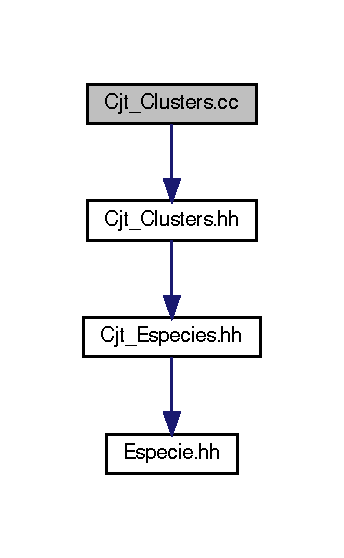
\includegraphics[width=165pt]{_cjt___clusters_8cc__incl}
\end{center}
\end{figure}
\subsection*{Funciones}
\begin{DoxyCompactItemize}
\item 
void \hyperlink{_cjt___clusters_8cc_a5cec9117fc9081104f0adb60b07b64e5}{imprimir\+\_\+tabla} (const map$<$ string, map$<$ string, double $>$ $>$ \&m)
\item 
void \hyperlink{_cjt___clusters_8cc_a4afe93558c94b1dce66fff0cf68cb08a}{imprimir\+\_\+preorden} (const Bin\+Tree$<$ pair$<$ string, double $>$ $>$ \&t)
\end{DoxyCompactItemize}


\subsection{Descripción detallada}
Código de la clase \hyperlink{class_cjt___clusters}{Cjt\+\_\+\+Clusters}. 



\subsection{Documentación de las funciones}
\mbox{\Hypertarget{_cjt___clusters_8cc_a5cec9117fc9081104f0adb60b07b64e5}\label{_cjt___clusters_8cc_a5cec9117fc9081104f0adb60b07b64e5}} 
\index{Cjt\+\_\+\+Clusters.\+cc@{Cjt\+\_\+\+Clusters.\+cc}!imprimir\+\_\+tabla@{imprimir\+\_\+tabla}}
\index{imprimir\+\_\+tabla@{imprimir\+\_\+tabla}!Cjt\+\_\+\+Clusters.\+cc@{Cjt\+\_\+\+Clusters.\+cc}}
\subsubsection{\texorpdfstring{imprimir\+\_\+tabla()}{imprimir\_tabla()}}
{\footnotesize\ttfamily void imprimir\+\_\+tabla (\begin{DoxyParamCaption}\item[{const map$<$ string, map$<$ string, double $>$ $>$ \&}]{m }\end{DoxyParamCaption})}



Definición en la línea 52 del archivo Cjt\+\_\+\+Clusters.\+cc.


\begin{DoxyCode}
52                                                                 \{
53   map<string, map<string, double> >::const\_iterator it1 = m.begin();
54   \textcolor{keywordflow}{while} (it1 != m.end()) \{
55     cout << it1->first << \textcolor{stringliteral}{":"};
56     map<string, double>::const\_iterator it2 = it1->second.begin();
57     \textcolor{keywordflow}{while} (it2 != it1->second.end()) \{
58       cout << \textcolor{stringliteral}{" "} << it2->first << \textcolor{stringliteral}{" ("} << it2->second << \textcolor{stringliteral}{")"};
59       ++it2;
60     \}
61     cout << endl;
62     ++it1;
63   \}
64 \}
\end{DoxyCode}
\mbox{\Hypertarget{_cjt___clusters_8cc_a4afe93558c94b1dce66fff0cf68cb08a}\label{_cjt___clusters_8cc_a4afe93558c94b1dce66fff0cf68cb08a}} 
\index{Cjt\+\_\+\+Clusters.\+cc@{Cjt\+\_\+\+Clusters.\+cc}!imprimir\+\_\+preorden@{imprimir\+\_\+preorden}}
\index{imprimir\+\_\+preorden@{imprimir\+\_\+preorden}!Cjt\+\_\+\+Clusters.\+cc@{Cjt\+\_\+\+Clusters.\+cc}}
\subsubsection{\texorpdfstring{imprimir\+\_\+preorden()}{imprimir\_preorden()}}
{\footnotesize\ttfamily void imprimir\+\_\+preorden (\begin{DoxyParamCaption}\item[{const Bin\+Tree$<$ pair$<$ string, double $>$ $>$ \&}]{t }\end{DoxyParamCaption})}



Definición en la línea 150 del archivo Cjt\+\_\+\+Clusters.\+cc.


\begin{DoxyCode}
150                                                                 \{
151 
152   \textcolor{keywordflow}{if} (not t.empty()) \{
153     cout << \textcolor{stringliteral}{"["};
154     \textcolor{keywordtype}{double} d = t.value().second;
155     \textcolor{keywordflow}{if} (d == -1) cout << t.value().first;
156     \textcolor{keywordflow}{else} cout << \textcolor{stringliteral}{"("} << t.value().first << \textcolor{stringliteral}{", "} << d << \textcolor{stringliteral}{") "};
157     \hyperlink{_cjt___clusters_8cc_a4afe93558c94b1dce66fff0cf68cb08a}{imprimir\_preorden}(t.left());
158     \hyperlink{_cjt___clusters_8cc_a4afe93558c94b1dce66fff0cf68cb08a}{imprimir\_preorden}(t.right());
159     cout << \textcolor{stringliteral}{"]"};
160   \}
161 \}
\end{DoxyCode}

\hypertarget{_cjt___clusters_8hh}{}\section{Referencia del Archivo Cjt\+\_\+\+Clusters.\+hh}
\label{_cjt___clusters_8hh}\index{Cjt\+\_\+\+Clusters.\+hh@{Cjt\+\_\+\+Clusters.\+hh}}


Especificación de la clase \hyperlink{class_cjt___clusters}{Cjt\+\_\+\+Clusters}.  


Dependencia gráfica adjunta para Cjt\+\_\+\+Clusters.\+hh\+:\nopagebreak
\begin{figure}[H]
\begin{center}
\leavevmode
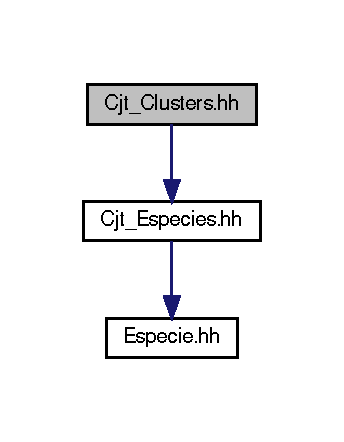
\includegraphics[width=165pt]{_cjt___clusters_8hh__incl}
\end{center}
\end{figure}
\subsection*{Clases}
\begin{DoxyCompactItemize}
\item 
class \hyperlink{class_cjt___clusters}{Cjt\+\_\+\+Clusters}
\begin{DoxyCompactList}\small\item\em Representa la información y las operaciones de un conjunto de clústers. \end{DoxyCompactList}\end{DoxyCompactItemize}


\subsection{Descripción detallada}
Especificación de la clase \hyperlink{class_cjt___clusters}{Cjt\+\_\+\+Clusters}. 


\hypertarget{_cjt___especies_8cc}{}\section{Referencia del Archivo Cjt\+\_\+\+Especies.\+cc}
\label{_cjt___especies_8cc}\index{Cjt\+\_\+\+Especies.\+cc@{Cjt\+\_\+\+Especies.\+cc}}


Código de la clase \hyperlink{class_cjt___especies}{Cjt\+\_\+\+Especies}.  


Dependencia gráfica adjunta para Cjt\+\_\+\+Especies.\+cc\+:\nopagebreak
\begin{figure}[H]
\begin{center}
\leavevmode
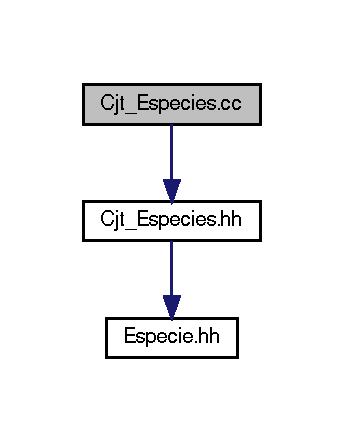
\includegraphics[width=165pt]{_cjt___especies_8cc__incl}
\end{center}
\end{figure}
\subsection*{Funciones}
\begin{DoxyCompactItemize}
\item 
void \hyperlink{_cjt___especies_8cc_aece33ee22015435a5dbac3d1f92ae2f5}{swap} (string \&a, string \&b)
\end{DoxyCompactItemize}


\subsection{Descripción detallada}
Código de la clase \hyperlink{class_cjt___especies}{Cjt\+\_\+\+Especies}. 



\subsection{Documentación de las funciones}
\mbox{\Hypertarget{_cjt___especies_8cc_aece33ee22015435a5dbac3d1f92ae2f5}\label{_cjt___especies_8cc_aece33ee22015435a5dbac3d1f92ae2f5}} 
\index{Cjt\+\_\+\+Especies.\+cc@{Cjt\+\_\+\+Especies.\+cc}!swap@{swap}}
\index{swap@{swap}!Cjt\+\_\+\+Especies.\+cc@{Cjt\+\_\+\+Especies.\+cc}}
\subsubsection{\texorpdfstring{swap()}{swap()}}
{\footnotesize\ttfamily void swap (\begin{DoxyParamCaption}\item[{string \&}]{a,  }\item[{string \&}]{b }\end{DoxyParamCaption})}



Definición en la línea 57 del archivo Cjt\+\_\+\+Especies.\+cc.


\begin{DoxyCode}
57                                 \{
58   \textcolor{keywordtype}{string} aux = a;
59   a = b;
60   b = aux;
61 \}
\end{DoxyCode}

\hypertarget{_cjt___especies_8hh}{}\section{Referencia del Archivo Cjt\+\_\+\+Especies.\+hh}
\label{_cjt___especies_8hh}\index{Cjt\+\_\+\+Especies.\+hh@{Cjt\+\_\+\+Especies.\+hh}}


Especificación de la clase \hyperlink{class_cjt___especies}{Cjt\+\_\+\+Especies}.  


Dependencia gráfica adjunta para Cjt\+\_\+\+Especies.\+hh\+:\nopagebreak
\begin{figure}[H]
\begin{center}
\leavevmode
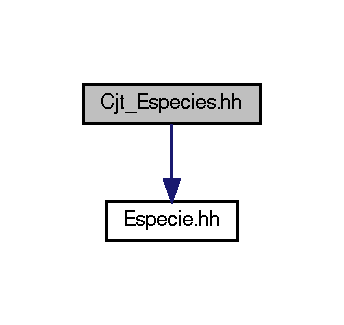
\includegraphics[width=165pt]{_cjt___especies_8hh__incl}
\end{center}
\end{figure}
\subsection*{Clases}
\begin{DoxyCompactItemize}
\item 
class \hyperlink{class_cjt___especies}{Cjt\+\_\+\+Especies}
\begin{DoxyCompactList}\small\item\em Representa la información y las operaciones asociadas a un conjunto de especies. \end{DoxyCompactList}\end{DoxyCompactItemize}


\subsection{Descripción detallada}
Especificación de la clase \hyperlink{class_cjt___especies}{Cjt\+\_\+\+Especies}. 


\hypertarget{_especie_8cc}{}\section{Referencia del Archivo Especie.\+cc}
\label{_especie_8cc}\index{Especie.\+cc@{Especie.\+cc}}


Código de la clase \hyperlink{class_especie}{Especie}.  


Dependencia gráfica adjunta para Especie.\+cc\+:\nopagebreak
\begin{figure}[H]
\begin{center}
\leavevmode
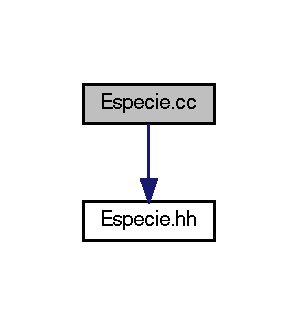
\includegraphics[width=143pt]{_especie_8cc__incl}
\end{center}
\end{figure}


\subsection{Descripción detallada}
Código de la clase \hyperlink{class_especie}{Especie}. 


\hypertarget{_especie_8hh}{}\section{Referencia del Archivo Especie.\+hh}
\label{_especie_8hh}\index{Especie.\+hh@{Especie.\+hh}}


Especificación de la clase \hyperlink{class_especie}{Especie}.  


\subsection*{Clases}
\begin{DoxyCompactItemize}
\item 
class \hyperlink{class_especie}{Especie}
\begin{DoxyCompactList}\small\item\em Representa la información y las operaciones asociadas a una especie. \end{DoxyCompactList}\end{DoxyCompactItemize}


\subsection{Descripción detallada}
Especificación de la clase \hyperlink{class_especie}{Especie}. 


\hypertarget{program_8cc}{}\section{Referencia del Archivo program.\+cc}
\label{program_8cc}\index{program.\+cc@{program.\+cc}}


Programa principal.  


Dependencia gráfica adjunta para program.\+cc\+:\nopagebreak
\begin{figure}[H]
\begin{center}
\leavevmode
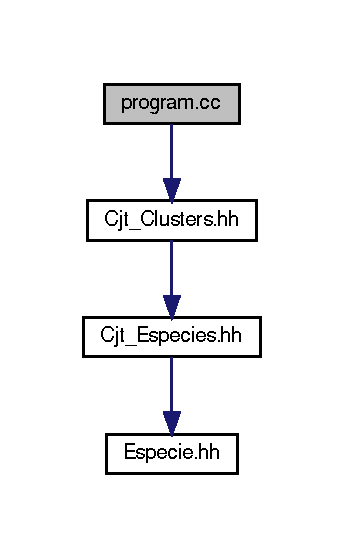
\includegraphics[width=165pt]{program_8cc__incl}
\end{center}
\end{figure}
\subsection*{Funciones}
\begin{DoxyCompactItemize}
\item 
int \hyperlink{program_8cc_ae66f6b31b5ad750f1fe042a706a4e3d4}{main} ()
\end{DoxyCompactItemize}


\subsection{Descripción detallada}
Programa principal. 

Estamos suponiendo que todos los datos de entrada cumplen el formato decidido en el enunciado de la práctica y, por lo tanto, son válidos, por lo que no se hace ninguna comprobación sobre estos. 

\subsection{Documentación de las funciones}
\mbox{\Hypertarget{program_8cc_ae66f6b31b5ad750f1fe042a706a4e3d4}\label{program_8cc_ae66f6b31b5ad750f1fe042a706a4e3d4}} 
\index{program.\+cc@{program.\+cc}!main@{main}}
\index{main@{main}!program.\+cc@{program.\+cc}}
\subsubsection{\texorpdfstring{main()}{main()}}
{\footnotesize\ttfamily int main (\begin{DoxyParamCaption}{ }\end{DoxyParamCaption})}



Definición en la línea 22 del archivo program.\+cc.


\begin{DoxyCode}
22            \{
23   \textcolor{keywordtype}{int} k; \textcolor{comment}{// Longitud de una subsecuencia de un gen}
24   cin >> k;
25   \hyperlink{class_cjt___especies}{Cjt\_Especies} e(k);
26   \hyperlink{class_cjt___clusters}{Cjt\_Clusters} c;
27   \textcolor{keywordtype}{string} command; \textcolor{comment}{// Código de operación}
28   cin >> command;
29   \textcolor{keywordflow}{while} (command != \textcolor{stringliteral}{"fin"}) \{
30     \textcolor{keywordtype}{string} id;
31     \textcolor{keywordtype}{bool} b;
32     \textcolor{keywordflow}{if} (command == \textcolor{stringliteral}{"crea\_especie"}) \{
33       \textcolor{keywordtype}{string} gen;
34       cin >> \textcolor{keywordtype}{id} >> gen;
35       cout << \textcolor{stringliteral}{"# "} << command << \textcolor{stringliteral}{" "} << \textcolor{keywordtype}{id} << \textcolor{stringliteral}{" "} << gen << endl;
36       e.crear\_especie(\textcolor{keywordtype}{id}, gen, b);
37       \textcolor{keywordflow}{if} (not b) cout << \textcolor{stringliteral}{"ERROR: La especie "} << \textcolor{keywordtype}{id} << \textcolor{stringliteral}{" ya existe."} << endl;
38     \}
39     \textcolor{keywordflow}{else} \textcolor{keywordflow}{if} (command == \textcolor{stringliteral}{"obtener\_gen"}) \{
40       cin >> id;
41       cout << \textcolor{stringliteral}{"# "} << command << \textcolor{stringliteral}{" "} << \textcolor{keywordtype}{id} << endl;
42       \textcolor{keywordtype}{string} s = e.obtener\_gen(\textcolor{keywordtype}{id});
43       \textcolor{keywordflow}{if} (s == \textcolor{stringliteral}{"-1"}) cout << \textcolor{stringliteral}{"ERROR: La especie "} << \textcolor{keywordtype}{id} << \textcolor{stringliteral}{" no existe."} << endl;
44       \textcolor{keywordflow}{else} cout << s << endl;
45     \}
46     \textcolor{keywordflow}{else} \textcolor{keywordflow}{if} (command == \textcolor{stringliteral}{"distancia"}) \{
47       \textcolor{keywordtype}{string} id2;
48       cin >> \textcolor{keywordtype}{id} >> id2;
49       cout << \textcolor{stringliteral}{"# "} << command << \textcolor{stringliteral}{" "} << \textcolor{keywordtype}{id} << \textcolor{stringliteral}{" "} << id2 << endl;
50       \textcolor{keywordtype}{double} d = e.consultar\_distancia(\textcolor{keywordtype}{id}, id2);
51       \textcolor{keywordflow}{if} (d == -1) cout << \textcolor{stringliteral}{"ERROR: La especie "} << \textcolor{keywordtype}{id} << \textcolor{stringliteral}{" no existe."} << endl;
52       \textcolor{keywordflow}{else} \textcolor{keywordflow}{if} (d == -2) cout << \textcolor{stringliteral}{"ERROR: La especie "} << id2 << \textcolor{stringliteral}{" no existe."} << endl;
53       \textcolor{keywordflow}{else} \textcolor{keywordflow}{if} (d == -3) cout << \textcolor{stringliteral}{"ERROR: La especie "} << \textcolor{keywordtype}{id} << \textcolor{stringliteral}{" y la especie "} << id2 << \textcolor{stringliteral}{" no existen."} << 
      endl;
54       \textcolor{keywordflow}{else} cout << d << endl;
55     \}
56     \textcolor{keywordflow}{else} \textcolor{keywordflow}{if} (command == \textcolor{stringliteral}{"elimina\_especie"}) \{
57       cin >> id;
58       cout << \textcolor{stringliteral}{"# "} << command << \textcolor{stringliteral}{" "} << \textcolor{keywordtype}{id} << endl;
59       e.eliminar\_especie(\textcolor{keywordtype}{id}, b);
60       \textcolor{keywordflow}{if} (not b) cout << \textcolor{stringliteral}{"ERROR: La especie "} << \textcolor{keywordtype}{id} << \textcolor{stringliteral}{" no existe."}  << endl;
61     \}
62     \textcolor{keywordflow}{else} \textcolor{keywordflow}{if} (command == \textcolor{stringliteral}{"existe\_especie"}) \{
63       cin >> id;
64       cout << \textcolor{stringliteral}{"# "} << command << \textcolor{stringliteral}{" "} << \textcolor{keywordtype}{id} << endl;
65       \textcolor{keywordtype}{bool} b = e.existe\_especie(\textcolor{keywordtype}{id});
66       \textcolor{keywordflow}{if} (b) cout << \textcolor{stringliteral}{"SI"} << endl;
67       \textcolor{keywordflow}{else} cout << \textcolor{stringliteral}{"NO"} << endl;
68     \}
69     \textcolor{keywordflow}{else} \textcolor{keywordflow}{if} (command == \textcolor{stringliteral}{"lee\_cjt\_especies"}) \{
70       cout << \textcolor{stringliteral}{"# "} << command << endl;
71       e = \hyperlink{class_cjt___especies}{Cjt\_Especies}(k);
72       e.leer\_cjt\_especies();
73       \}
74     \textcolor{keywordflow}{else} \textcolor{keywordflow}{if} (command == \textcolor{stringliteral}{"imprime\_cjt\_especies"}) \{
75       cout << \textcolor{stringliteral}{"# "} << command << endl;
76       e.imprimir\_cjt\_especies();
77     \}
78     \textcolor{keywordflow}{else} \textcolor{keywordflow}{if} (command == \textcolor{stringliteral}{"tabla\_distancias"}) \{
79       cout << \textcolor{stringliteral}{"# "} << command << endl;
80       e.imprimir\_distancias\_e();
81     \}
82     \textcolor{keywordflow}{else} \textcolor{keywordflow}{if} (command == \textcolor{stringliteral}{"inicializa\_clusters"}) \{
83       cout << \textcolor{stringliteral}{"# "} << command << endl;
84       c = \hyperlink{class_cjt___clusters}{Cjt\_Clusters}(e);
85       c.\hyperlink{class_cjt___clusters_a8caa8d4eae15730feccea2ce7d22a196}{imprimir\_distancias\_c}();
86     \}
87     \textcolor{keywordflow}{else} \textcolor{keywordflow}{if} (command == \textcolor{stringliteral}{"ejecuta\_paso\_wpgma"}) \{
88       cout << \textcolor{stringliteral}{"# "} << command << endl;
89       c.\hyperlink{class_cjt___clusters_a4675196f92740eda90fcbdf7942ee04b}{ejecutar\_paso\_wpgma}(b);
90       \textcolor{keywordflow}{if} (not b) cout << \textcolor{stringliteral}{"ERROR: num\_clusters <= 1"} << endl;
91     \}
92     \textcolor{keywordflow}{else} \textcolor{keywordflow}{if} (command == \textcolor{stringliteral}{"imprime\_cluster"}) \{
93       cin >> id;
94       cout << \textcolor{stringliteral}{"# "} << command << \textcolor{stringliteral}{" "} << \textcolor{keywordtype}{id} << endl;
95       c.\hyperlink{class_cjt___clusters_add140d48281573802396c267f0d15cee}{imprimir\_cluster}(\textcolor{keywordtype}{id}, b);
96       \textcolor{keywordflow}{if} (not b) cout << \textcolor{stringliteral}{"ERROR: El cluster "} << \textcolor{keywordtype}{id} << \textcolor{stringliteral}{" no existe."} << endl;
97     \}
98     \textcolor{keywordflow}{else} \textcolor{keywordflow}{if} (command == \textcolor{stringliteral}{"imprime\_arbol\_filogenetico"}) \{
99       cout << \textcolor{stringliteral}{"# "} << command << endl;
100       c = \hyperlink{class_cjt___clusters}{Cjt\_Clusters}(e);
101       c.\hyperlink{class_cjt___clusters_a289dfd3307b383620edc1f901dced7b0}{imprimir\_arbol\_filogenetico}(b);
102       \textcolor{keywordflow}{if} (b) cout << \textcolor{stringliteral}{"ERROR: El conjunto de clusters es vacio."} << endl;
103     \}
104     cout << endl;
105     cin >> command;
106   \}
107 \}
\end{DoxyCode}

%--- End generated contents ---

% Index
\backmatter
\newpage
\phantomsection
\clearemptydoublepage
\addcontentsline{toc}{chapter}{Índice}
\printindex

\end{document}
